\section{False Positive Rates versus Model Scaling}
\label{app:hall_scal}


% \begin{figure}[H]
%     \centering

%     % First row (2 centered subfigures)
%     \begin{minipage}{0.8\textwidth} 
%         \centering
%         \begin{subfigure}{0.45\textwidth}
%             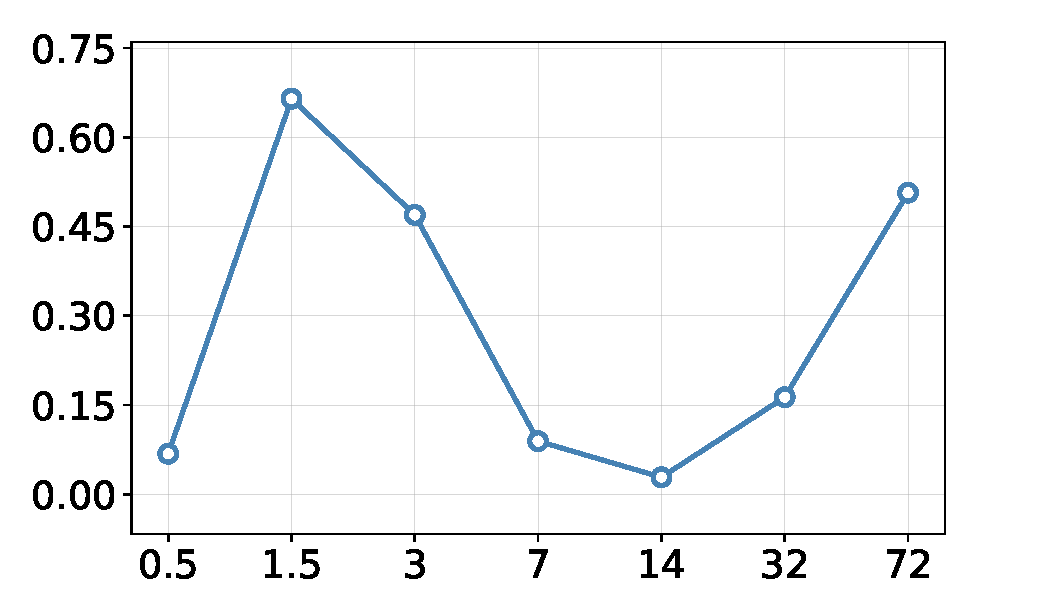
\includegraphics[width=\linewidth]{Figures_Qwen_scaling/Multi-subject-RLVR__mean.pdf}
%             \caption{Multi-subject RLVR Dataset}
%             \label{fig:sub1}
%         \end{subfigure}
%         \hfill
%         \begin{subfigure}{0.45\textwidth}
%             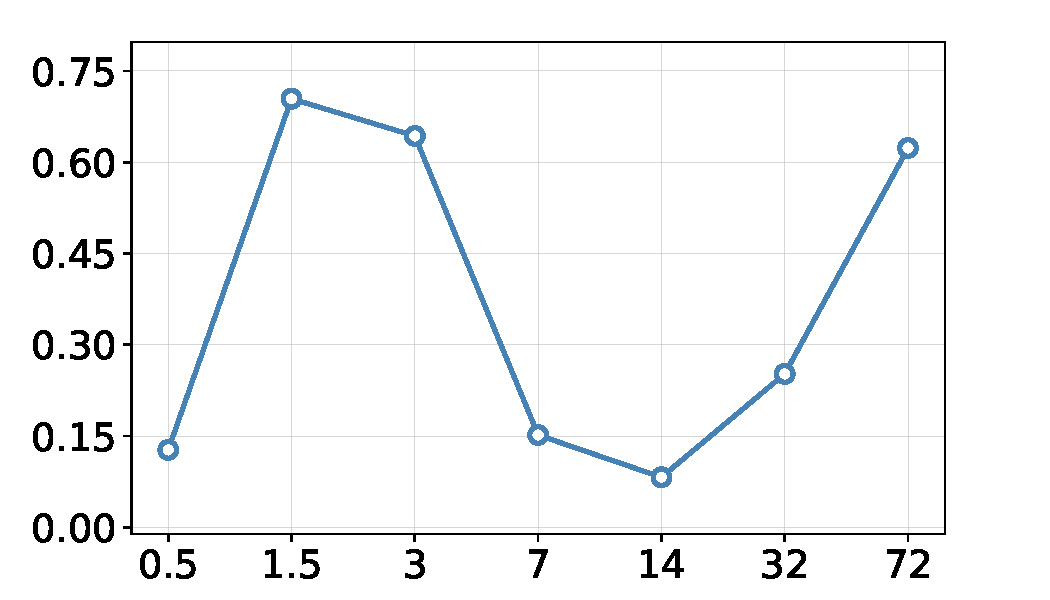
\includegraphics[width=\linewidth]{Figures_Qwen_scaling/Natural_Reasoning__mean.pdf}
%             \caption{NaturalReasoning Dataset}
%             \label{fig:sub2}
%         \end{subfigure}
%     \end{minipage}


%     \vspace{0.5em} % 
    
%     % second row (3)
%     \begin{subfigure}{0.32\textwidth}
%         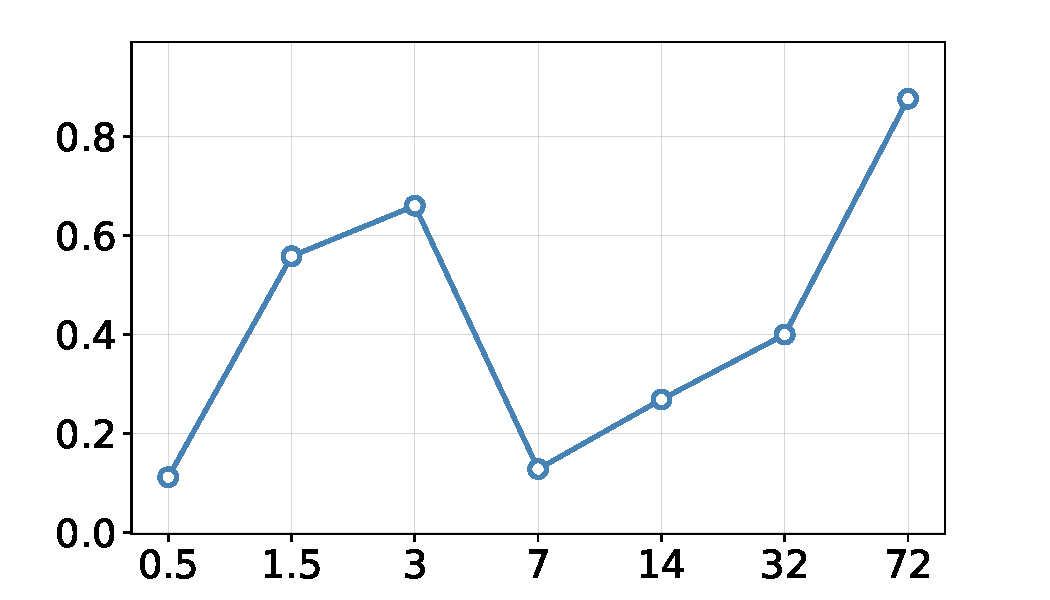
\includegraphics[width=\linewidth]{Figures_Qwen_scaling/GSM8k__mean.pdf}
%         \caption{GSM8K Dataset}
%         \label{fig:sub3}
%     \end{subfigure}
%     \hfill
%     \begin{subfigure}{0.32\textwidth}
%         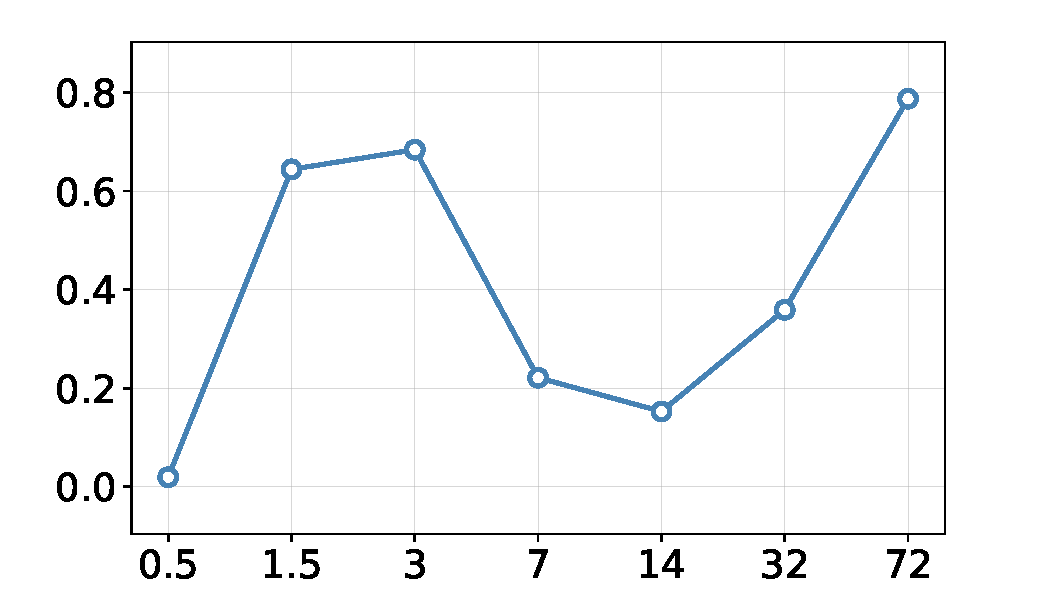
\includegraphics[width=\linewidth]{Figures_Qwen_scaling/MATH__mean.pdf}
%         \caption{MATH Dataset}
%         \label{fig:sub4}
%     \end{subfigure}
%     \hfill
%     \begin{subfigure}{0.32\textwidth}
%         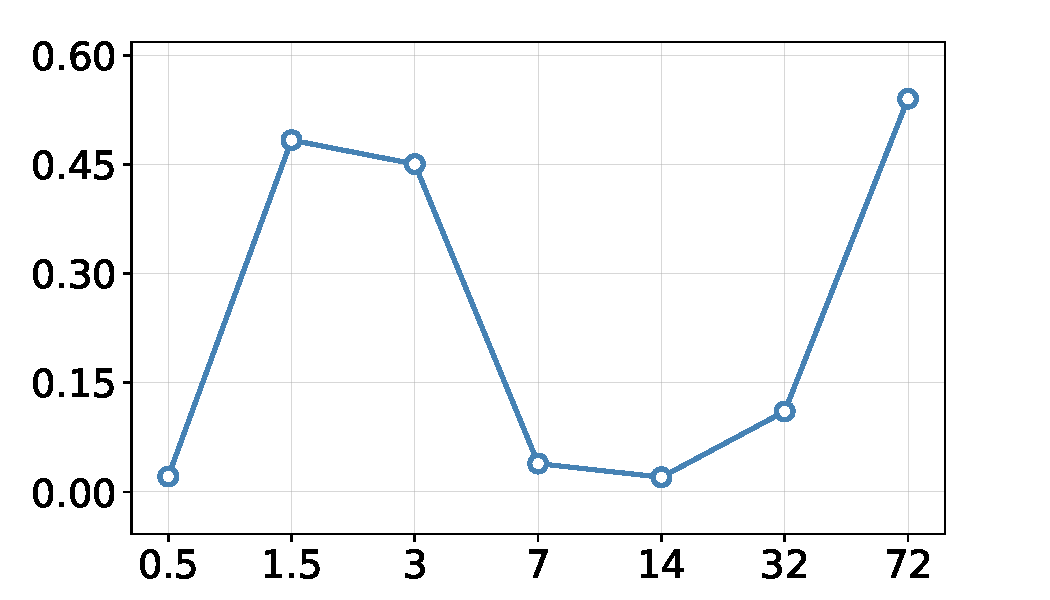
\includegraphics[width=\linewidth]{Figures_Qwen_scaling/AIME1983-2024__mean.pdf}
%         \caption{AIME1983-2024 Dataset}
%         \label{fig:sub5}
%     \end{subfigure}
    
%     \caption{\textbf{False positive rate (FPR) versus scaling of Qwen models.}  We evaluate the FPRs of the Qwen2.5-Instruct model series (with sizes 0.5B, 1.5B, 3B, 7B, 14B, 32B, and 72B) and analyze how FPR varies with model size. In all figures above, X-axis is model size (B) and y-axis is FPR averaged over all the ten ``master keys'' listed in Table~\ref{tab:merged-five}.}
%     \label{fig:Qwen-scaling}
% \end{figure}

We examined the scaling behavior of the Qwen2.5-Instruct model family (ranging from 0.5B to 72B parameters) across multiple benchmarks. Figure~\ref{fig:Qwen-scaling-main} reports the averaged scaling trend over the ten “master keys” listed in Table~\ref{tab:merged-five}. For completeness, we also present the scaling curves of each individual “master key” on the five benchmarks considered. In particular, the Multi-subject RLVR results are shown in Figure~\ref{fig:ten_multi_sub}, while Figures~\ref{fig:ten_natural_reason}, \ref{fig:ten_gsm8k}, \ref{fig:ten_math}, and \ref{fig:ten_aime} depict the corresponding behaviors on NaturalReasoning, GSM8K, MATH, and AIME1983–2024, respectively.

Surprisingly, the scaling patterns are consistent across all datasets and ``master keys'', but exhibit a non-monotonic trend. The 0.5B model achieves the lowest FPR but also shows the weakest alignment with GPT-4o (Table~\ref{tab:consistency}). As the model size increases to 1.5–3B, FPR rises sharply while consistency improves. Performance reaches its peak at 7–14B, balancing low FPR with high consistency, before FPR climbs again at the largest scales of 32B and 72B.

% In this section, we plot the scaling behavior of the Qwen2.5-Instruct model series (0.5B, 1.5B, 3B, 7B, 14B, 32B, 72B) across various ``master key'' responses and benchmarks. Figure~\ref{fig:ten_multi_sub} illustrates the scaling trends on the Multi-subject RLVR benchmark, while Figures~\ref{fig:ten_natural_reason}, \ref{fig:ten_gsm8k}, \ref{fig:ten_math}, and \ref{fig:ten_aime} show results for the NaturalReasoning, GSM8K, MATH, and AIME1983–2024 benchmarks, respectively.

% Across all benchmarks and responses, we observe a consistent non-monotonic scaling pattern: false positive rates initially rise from 0.5B to 1.5B and 3B, decrease at 7B and 14B, and rise again at 32B and 72B.

% We analyze how FPR varies with model size across the Qwen2.5-Instruct series, as shown in Figure \ref{fig:Qwen-scaling}. Surprisingly, the scaling behavior is consistent for all datasets but non-monotonic. The 0.5 B model exhibits the lowest FPR rate but also the weakest agreement with GPT-4o (Table~\ref{tab:consistency}). As model size increases to 1.5–3 B, FPR rises sharply while consistency improves. Performance then peaks at 7–14 B, achieving both low FPR and high consistency, before FPR increases again at the largest scales of 32 B and 72 B. 

We hypothesize the following mechanisms: (1) $0.5$ B (literal matcher): With limited knowledge, the model relies on surface-level string differences and therefore outputs NO whenever obvious mismatches appear, yielding lower FPR but many disagreements with GPT-4o.
(2) $1.5$ B/$3$ B (coarse semantic matcher): These models possess just enough capacity to detect embedding-level similarity (e.g., shared units, symbols, or synonyms), yet lack fine-grained verification; as a result, they tend to over-predict \texttt{YES} and produce frequent false positive judgments.
(3) $7$ B/$14$ B (calibrated verifier): Sufficient capacity enables precise comparison while retained caution suppresses unwarranted YES responses, producing the best overall trade-off.
(4) $32$ B/$72$ B (self-solver):  An observation was made that Claude-4 sometimes deviates from the provided instruction to compare a given solution with a reference answer. Instead, it solves the question independently and subsequently compares the reference answer to its own derived solution. While this behavior is infrequently observed in other models, we hypothesize that the increased false positive rate in larger models is attributable to their inherent tendency to solve the question themselves before comparing the reference answer to their own derivation, rather than the provided solution. As a partial validation of this hypothesis, we discovered that removing the question from the prompt (i.e., providing only a response and a reference answer for evaluation) significantly reduces the FPR. This effect is particularly pronounced in large models (see Appendix \ref{app:remove} for further details). We leave the further investigation of the mechanism behind this scaling behavior as a direction for future work.





\begin{figure*}[htbp]
    \centering
    % first row
    \begin{subfigure}{0.3\textwidth}
        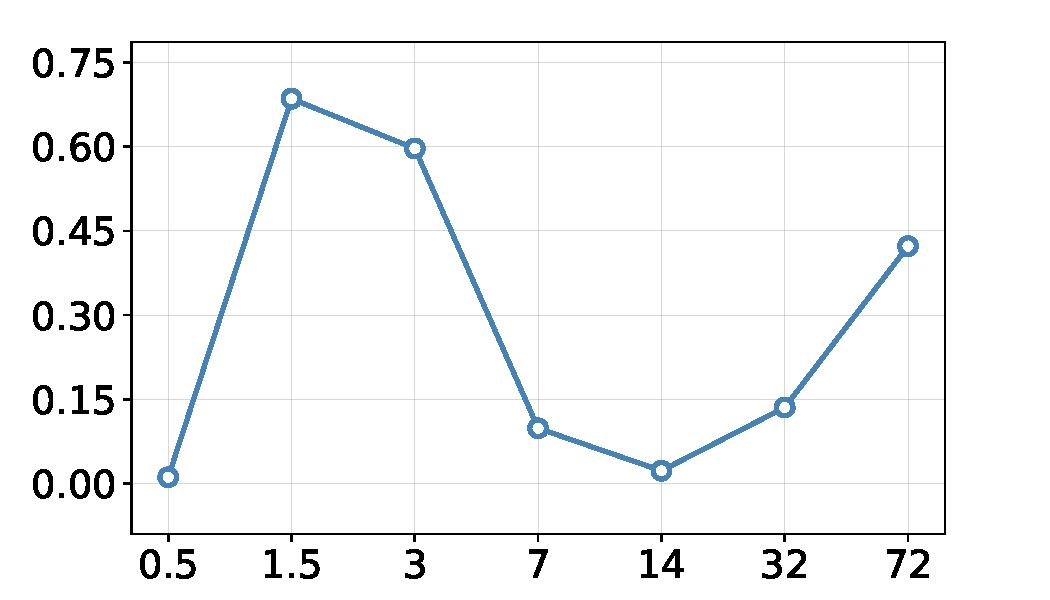
\includegraphics[width=\linewidth]{Figures_Qwen_scaling/Multi-subject-RLVR___.pdf}
        \caption{Resp. = " "}
    \end{subfigure}
    \hfill
    \begin{subfigure}{0.3\textwidth}
        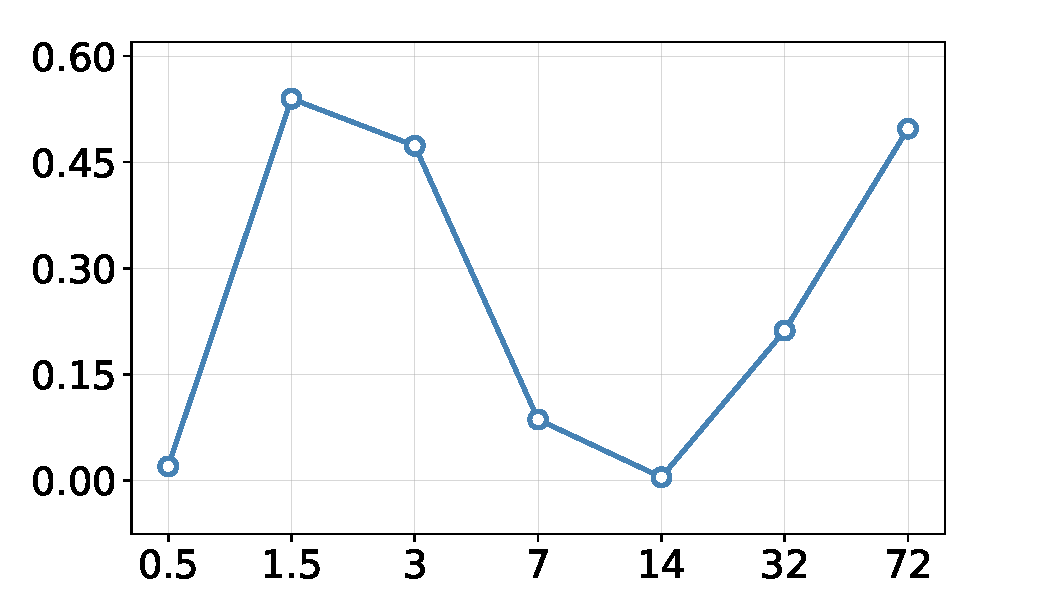
\includegraphics[width=\linewidth]{Figures_Qwen_scaling/Multi-subject-RLVR__..pdf}
        \caption{Resp. = "."}
    \end{subfigure}
    \hfill
    \begin{subfigure}{0.3\textwidth}
        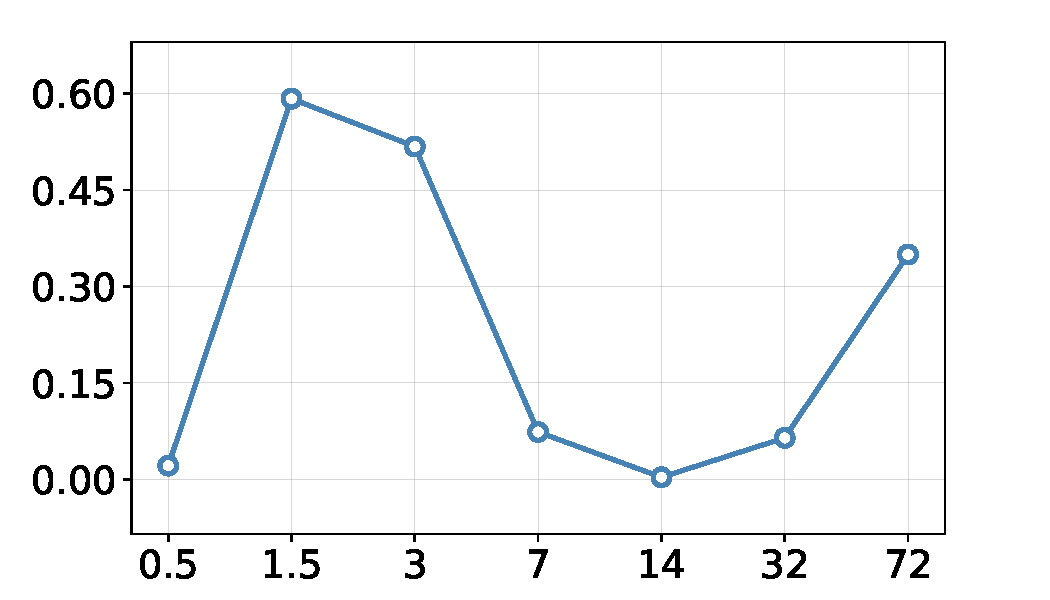
\includegraphics[width=\linewidth]{Figures_Qwen_scaling/Multi-subject-RLVR__,.pdf}
        \caption{Resp. = ","}
    \end{subfigure}
    
    \vspace{0.5em}
    % second row
    \begin{subfigure}{0.3\textwidth}
        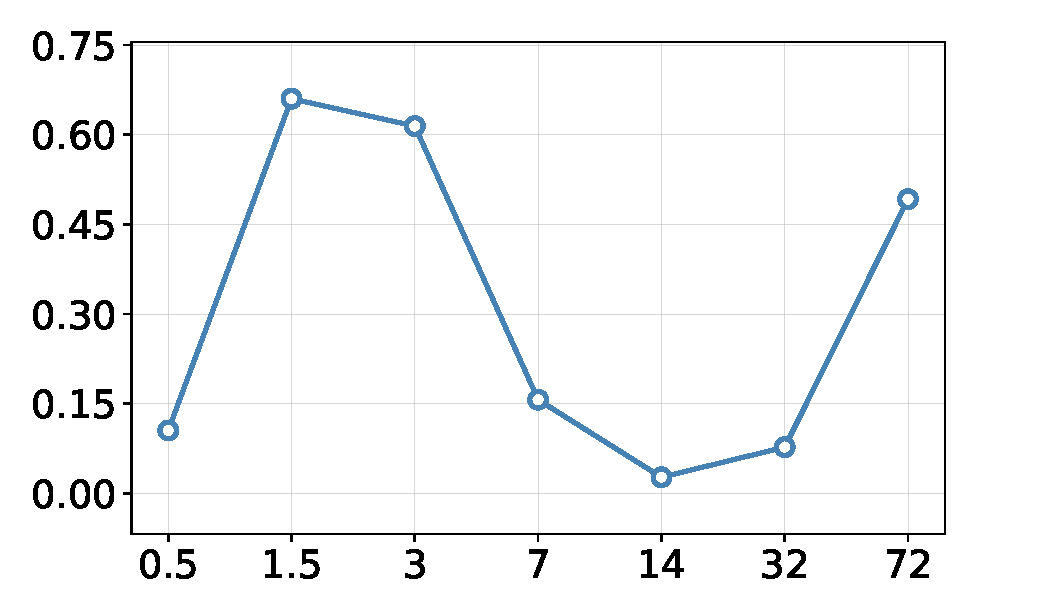
\includegraphics[width=\linewidth]{Figures_Qwen_scaling/Multi-subject-RLVR__colon.pdf}
        \caption{Resp. = ":"}
    \end{subfigure}
    \hfill
    \begin{subfigure}{0.3\textwidth}
        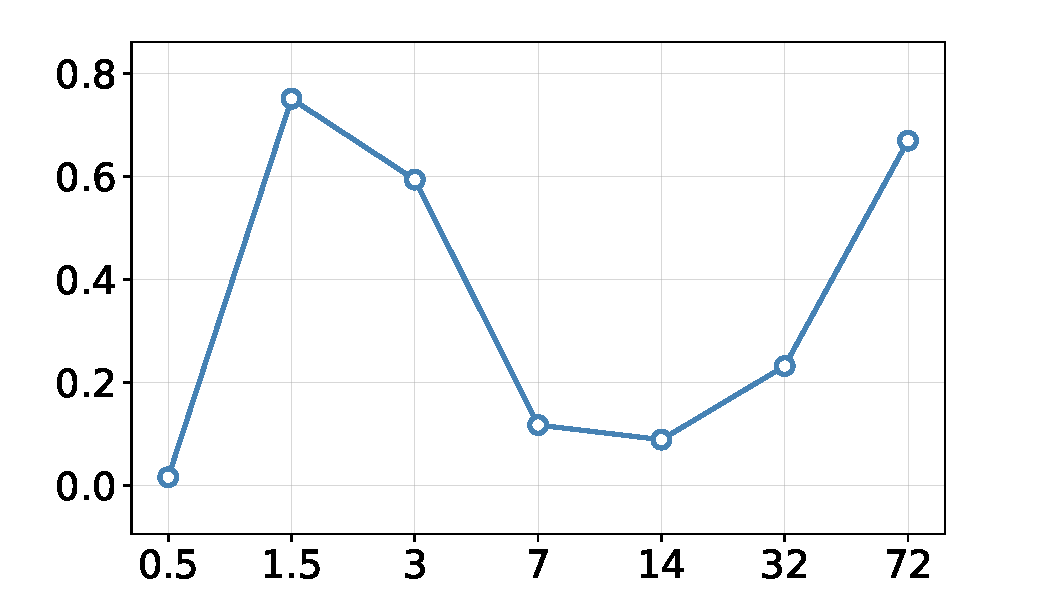
\includegraphics[width=\linewidth]{Figures_Qwen_scaling/Multi-subject-RLVR__Thought_processcolon.pdf}
        \caption{Resp. = "Thought process:"}
    \end{subfigure}
    \hfill
    \begin{subfigure}{0.3\textwidth}
        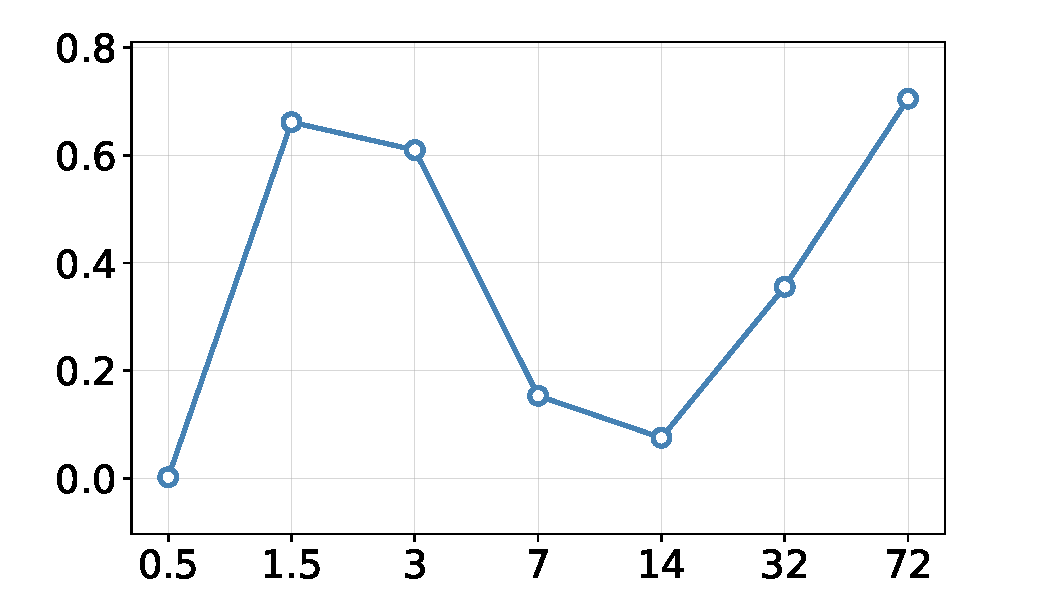
\includegraphics[width=\linewidth]{Figures_Qwen_scaling/Multi-subject-RLVR__Let_solve_this_problem_step_by_step..pdf}
        \caption{Resp. = "Let's solve this problem step by step"}
    \end{subfigure}
    
    \vspace{0.5em}
    % third row
    \begin{subfigure}{0.22\textwidth}
        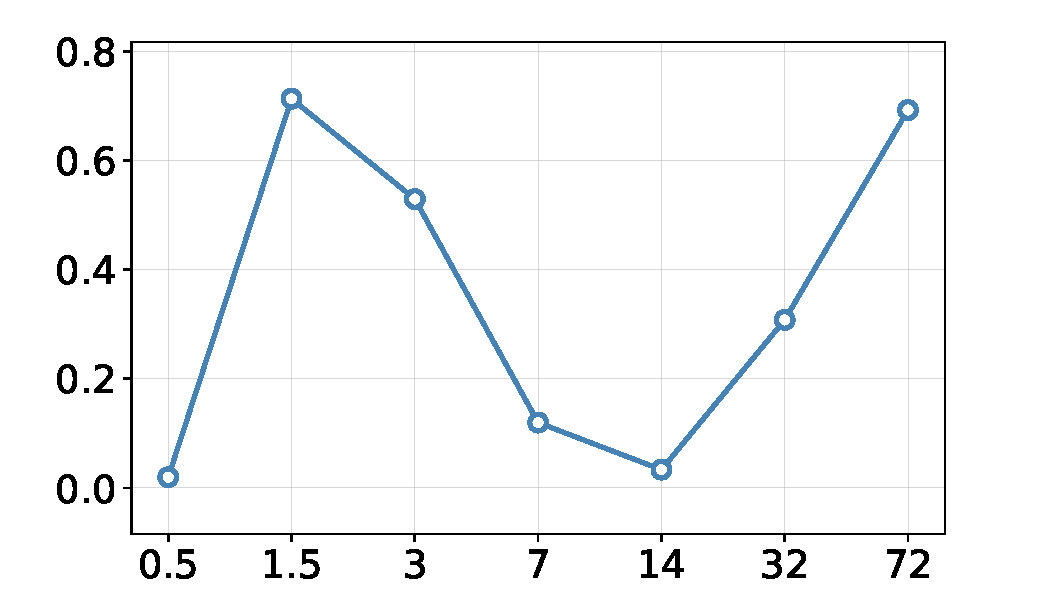
\includegraphics[width=\linewidth]{Figures_Qwen_scaling/Multi-subject-RLVR__Solution.pdf}
        \caption{Resp. = "Solution"}
    \end{subfigure}
    \hfill
    \begin{subfigure}{0.22\textwidth}
        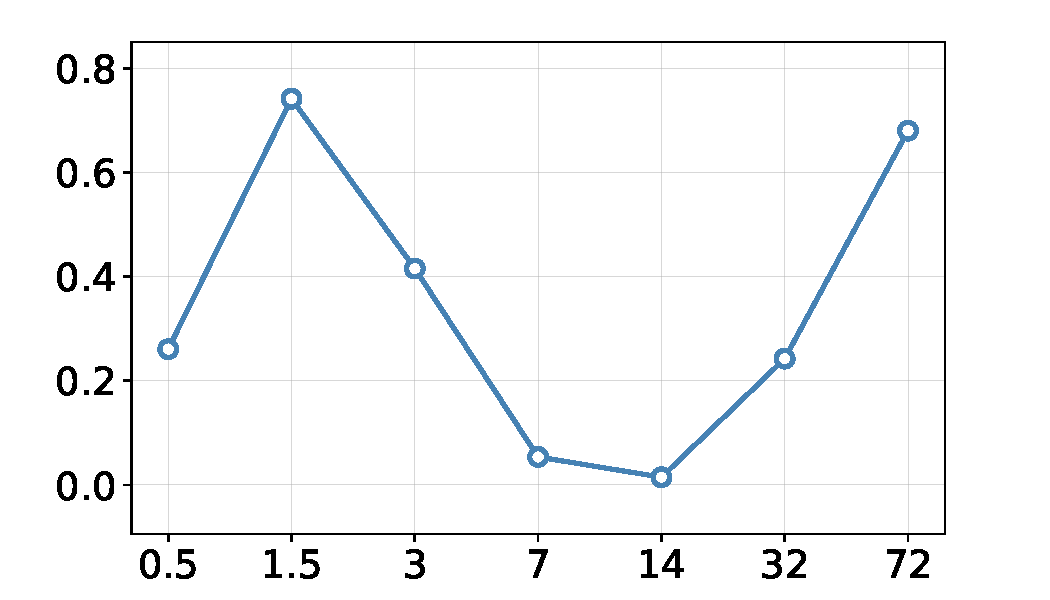
\includegraphics[width=\linewidth]{Figures_Qwen_scaling/Multi-subject-RLVR__china.pdf}
        \caption{Resp. = "\begin{CJK}{UTF8}{gbsn}解\end{CJK}"}
    \end{subfigure}
    \hfill
    \begin{subfigure}{0.22\textwidth}
        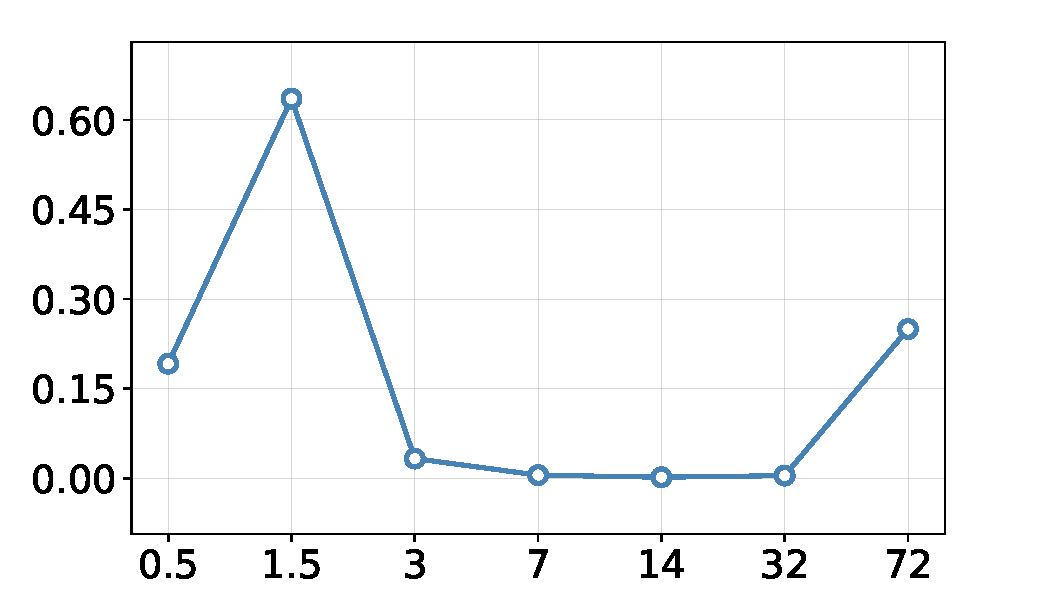
\includegraphics[width=\linewidth]{Figures_Qwen_scaling/Multi-subject-RLVR__jap.pdf}
        \caption{Resp. = \begin{CJK}{UTF8}{min}かいせつ\end{CJK}}
    \end{subfigure}
    \hfill
    \begin{subfigure}{0.22\textwidth}
        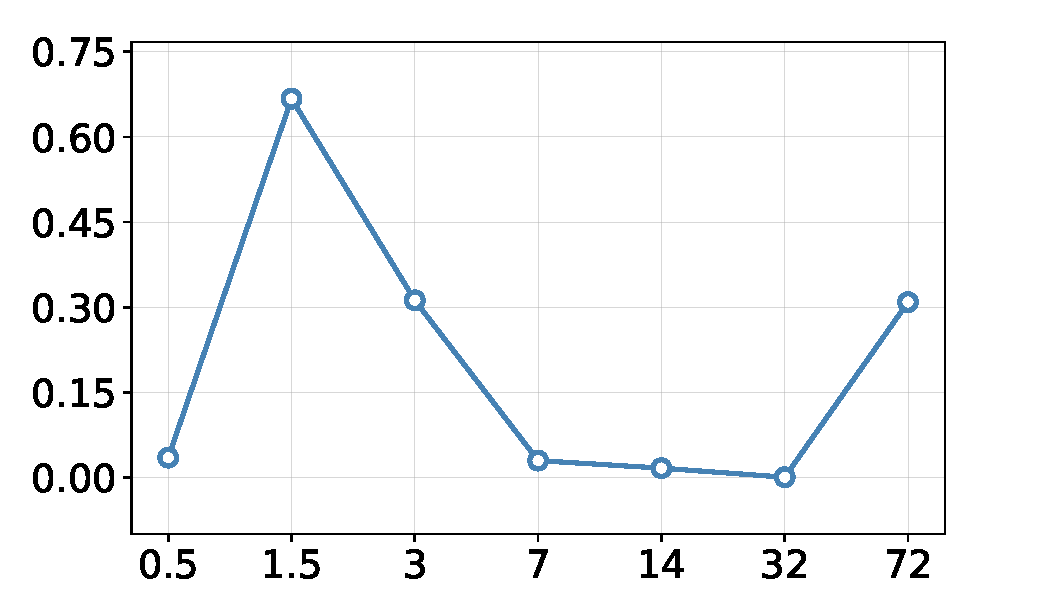
\includegraphics[width=\linewidth]{Figures_Qwen_scaling/Multi-subject-RLVR__Respuesta.pdf}
        \caption{Resp. = \foreignlanguage{spanish}{Respuesta}}
    \end{subfigure}
    
    \caption{Multi-subject RLVR Benchmark}
    \label{fig:ten_multi_sub}
\end{figure*}




\begin{figure*}[htbp]
    \centering
    % first row
    \begin{subfigure}{0.3\textwidth}
        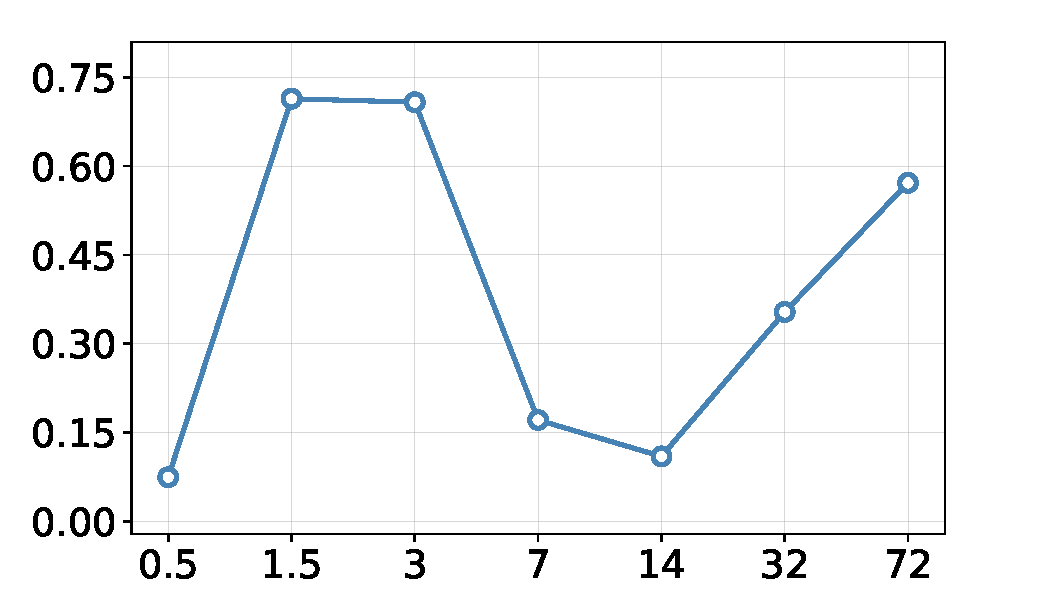
\includegraphics[width=\linewidth]{Figures_Qwen_scaling/Natural_Reasoning___.pdf}
        \caption{Resp. = " "}
    \end{subfigure}
    \hfill
    \begin{subfigure}{0.3\textwidth}
        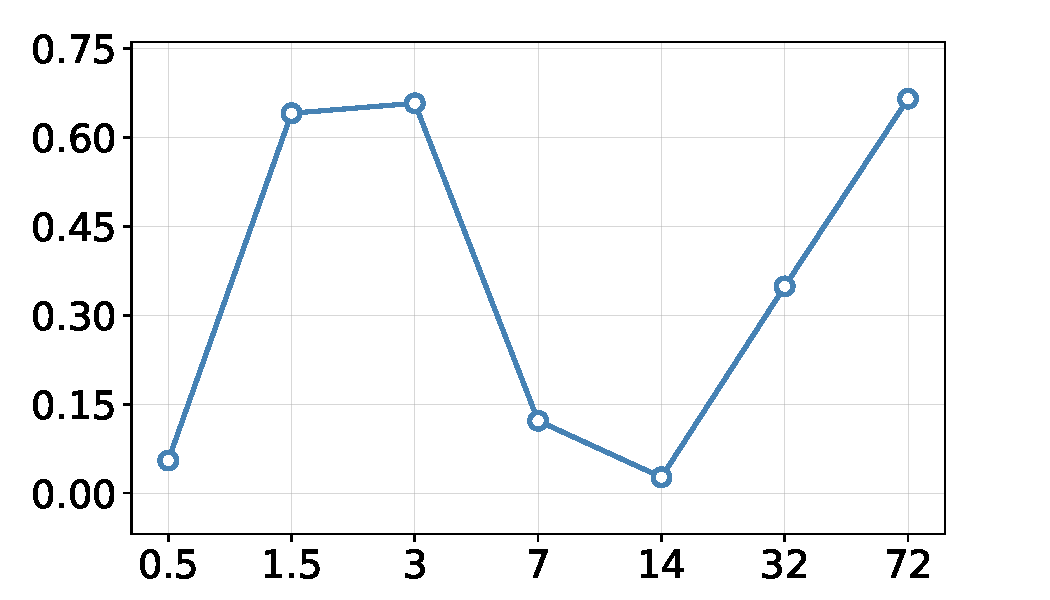
\includegraphics[width=\linewidth]{Figures_Qwen_scaling/Natural_Reasoning__..pdf}
        \caption{Resp. = "."}
    \end{subfigure}
    \hfill
    \begin{subfigure}{0.3\textwidth}
        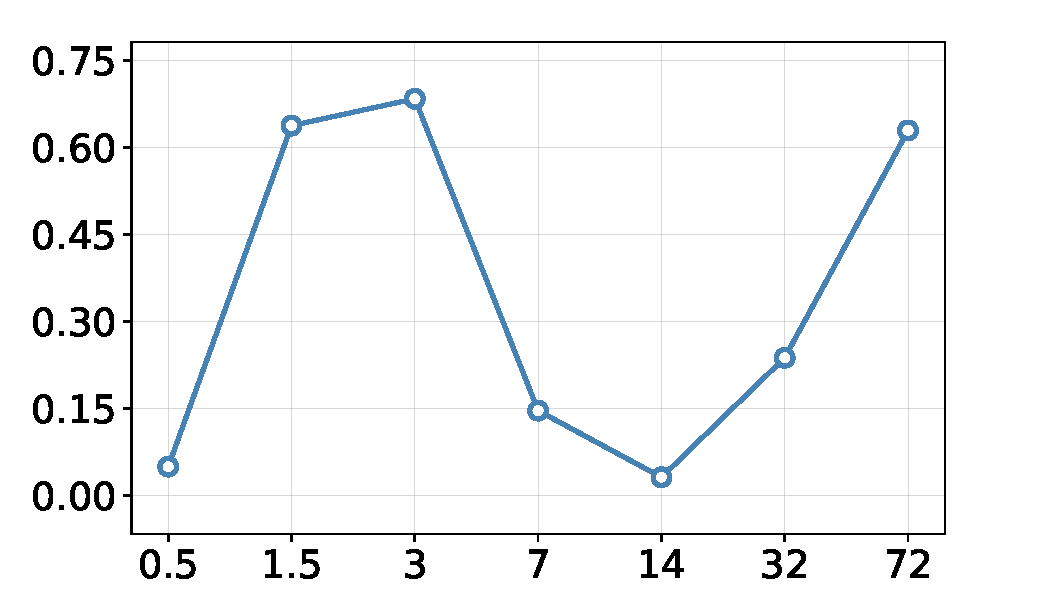
\includegraphics[width=\linewidth]{Figures_Qwen_scaling/Natural_Reasoning__,.pdf}
        \caption{Resp. = ","}
    \end{subfigure}
    
    \vspace{0.5em}
    % second row
    \begin{subfigure}{0.3\textwidth}
        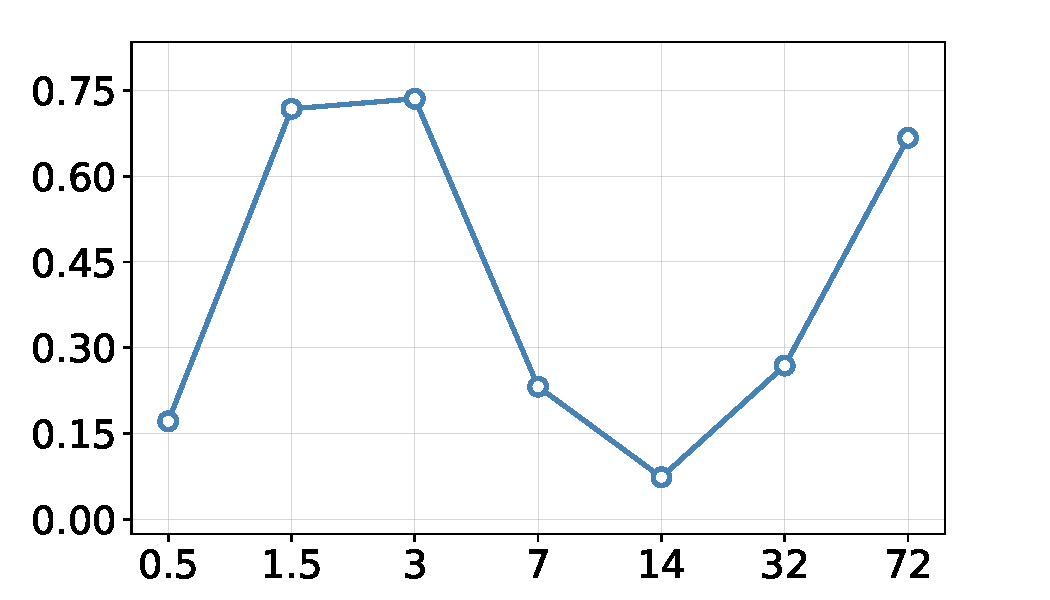
\includegraphics[width=\linewidth]{Figures_Qwen_scaling/Natural_Reasoning__colon.pdf}
        \caption{Resp. = ":"}
    \end{subfigure}
    \hfill
    \begin{subfigure}{0.3\textwidth}
        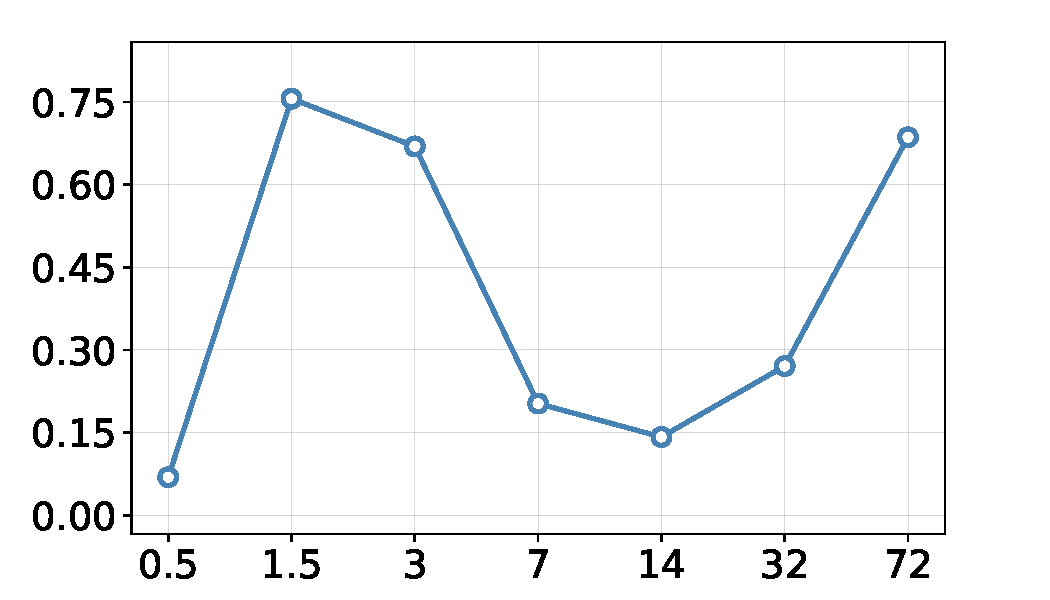
\includegraphics[width=\linewidth]{Figures_Qwen_scaling/Natural_Reasoning__Thought_processcolon.pdf}
        \caption{Resp. = "Thought process:"}
    \end{subfigure}
    \hfill
    \begin{subfigure}{0.3\textwidth}
        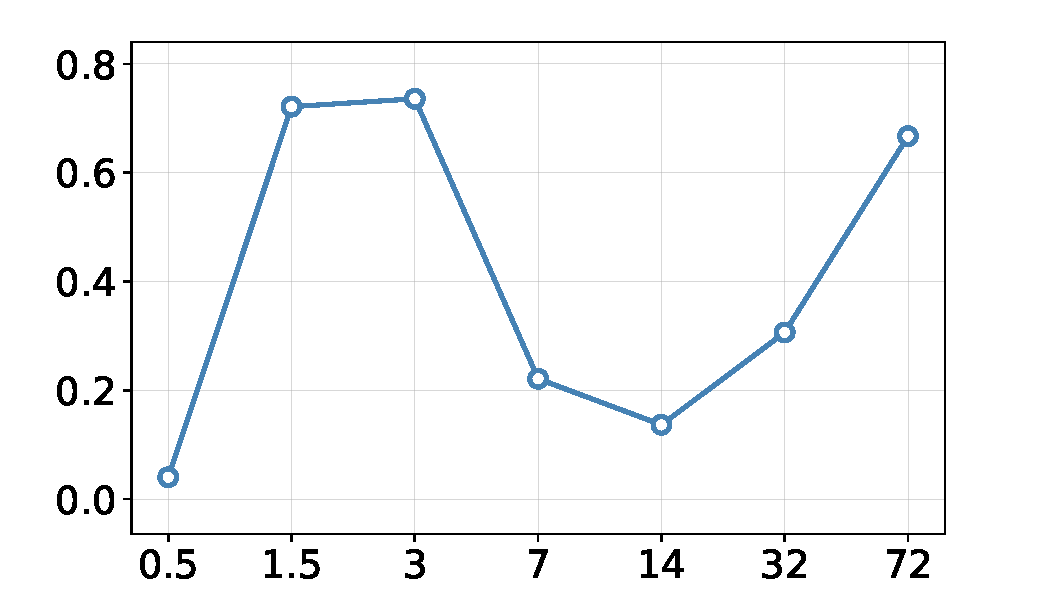
\includegraphics[width=\linewidth]{Figures_Qwen_scaling/Natural_Reasoning__Let_solve_this_problem_step_by_step..pdf}
        \caption{Resp. = "Let's solve this problem step by step"}
    \end{subfigure}
    
    \vspace{0.5em}
    % third row
    \begin{subfigure}{0.22\textwidth}
        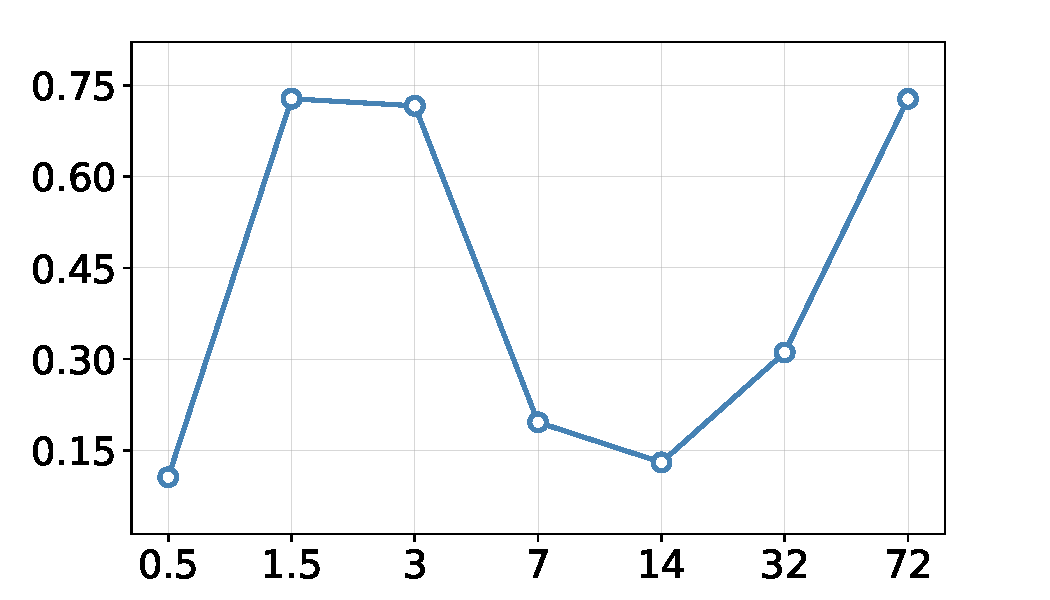
\includegraphics[width=\linewidth]{Figures_Qwen_scaling/Natural_Reasoning__Solution.pdf}
        \caption{Resp. = "Solution"}
    \end{subfigure}
    \hfill
    \begin{subfigure}{0.22\textwidth}
        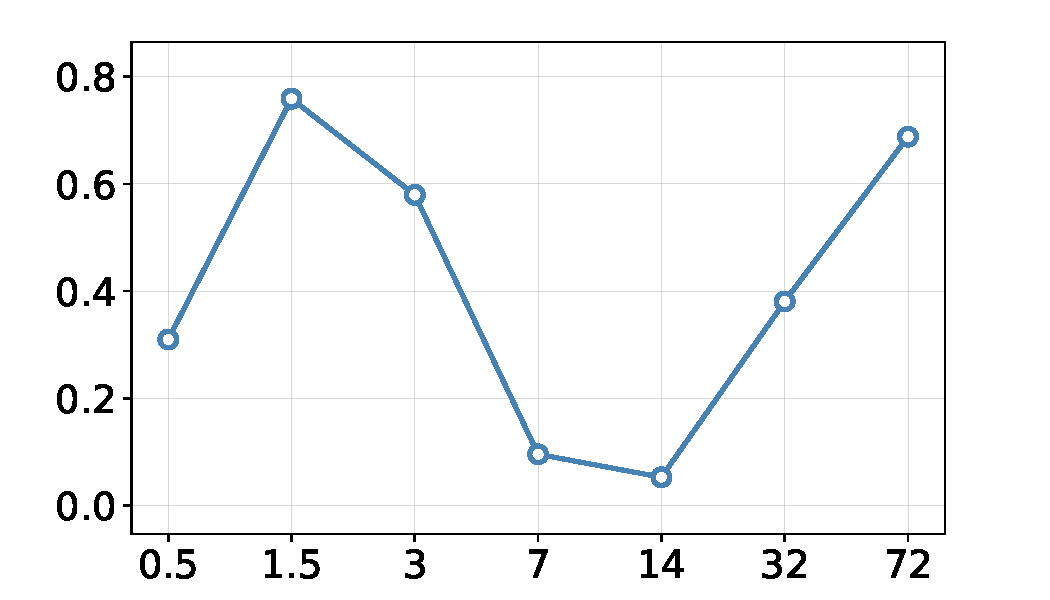
\includegraphics[width=\linewidth]{Figures_Qwen_scaling/Natural_Reasoning__china.pdf}
        \caption{Resp. = "\begin{CJK}{UTF8}{gbsn}解\end{CJK}"}
    \end{subfigure}
    \hfill
    \begin{subfigure}{0.22\textwidth}
        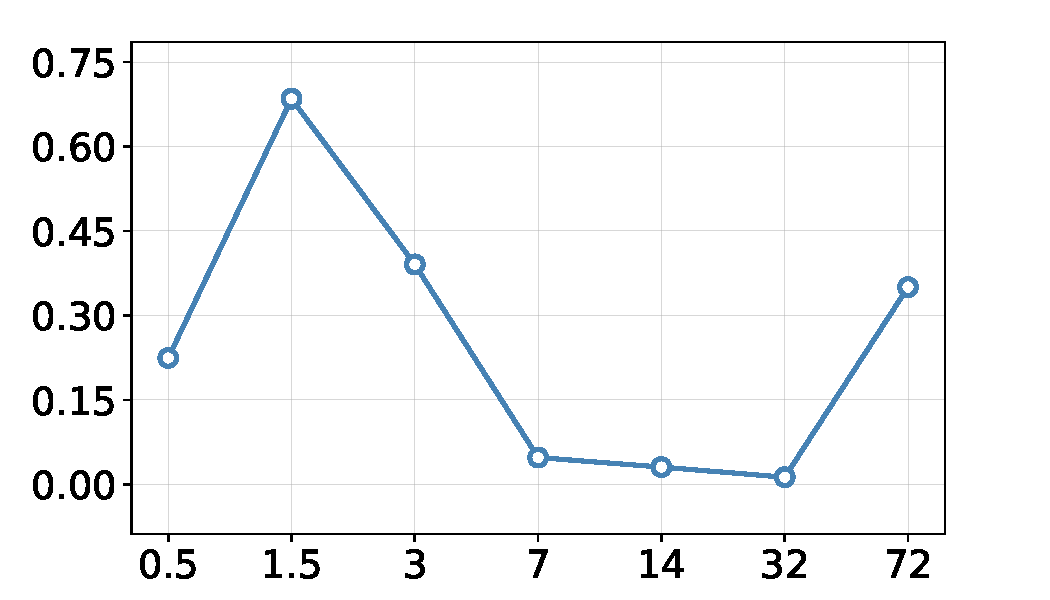
\includegraphics[width=\linewidth]{Figures_Qwen_scaling/Natural_Reasoning__jap.pdf}
        \caption{Resp. = \begin{CJK}{UTF8}{min}かいせつ\end{CJK}}
    \end{subfigure}
    \hfill
    \begin{subfigure}{0.22\textwidth}
        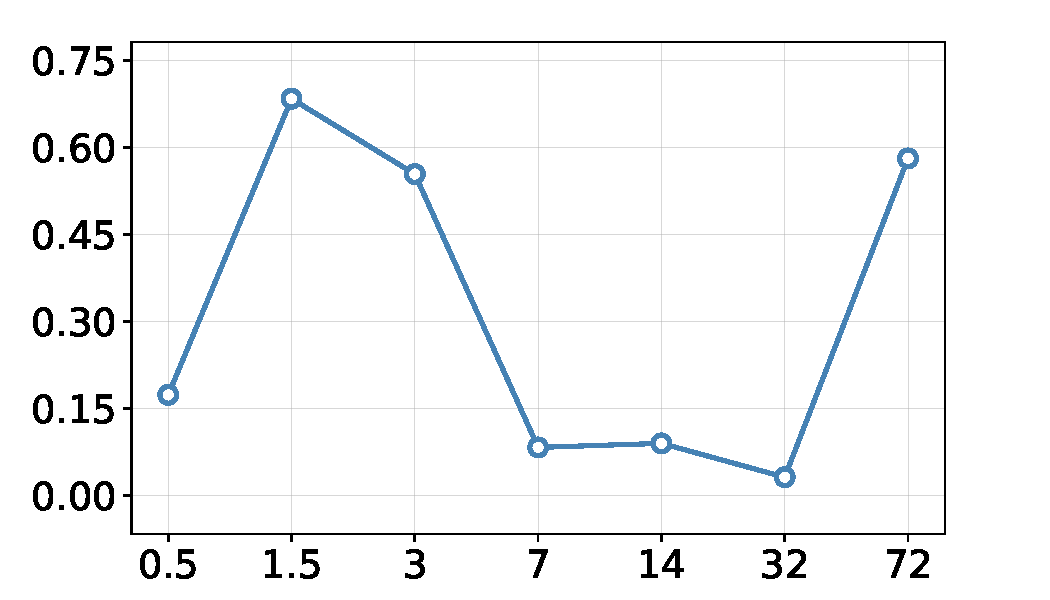
\includegraphics[width=\linewidth]{Figures_Qwen_scaling/Natural_Reasoning__Respuesta.pdf}
        \caption{Resp. = \foreignlanguage{spanish}{Respuesta}}
    \end{subfigure}
    
    \caption{NaturalReasoning Benchmark}
    \label{fig:ten_natural_reason}
\end{figure*}


\begin{figure*}[htbp]
    \centering
    % first row
    \begin{subfigure}{0.3\textwidth}
        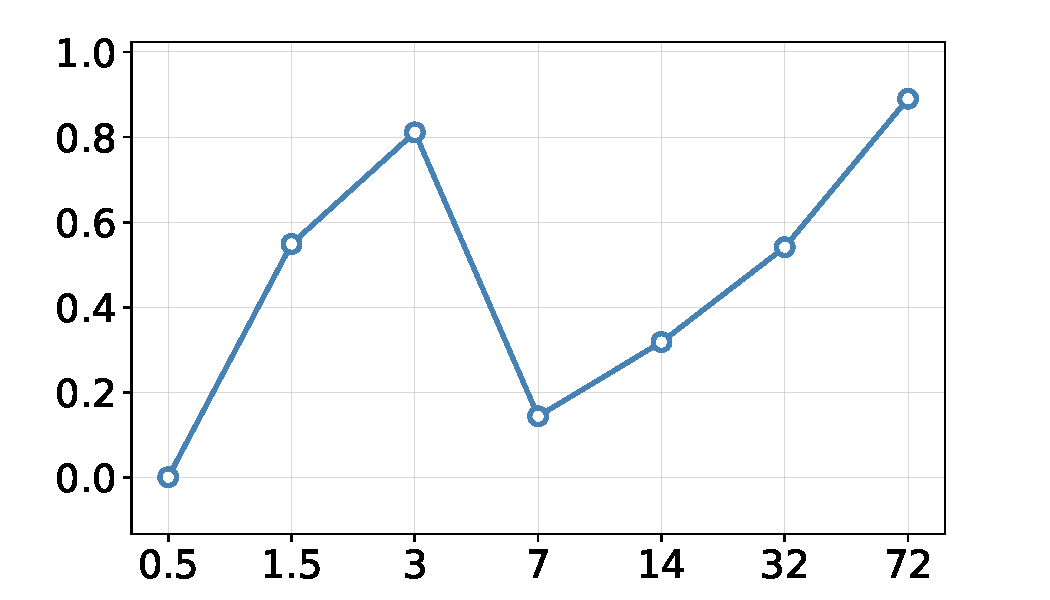
\includegraphics[width=\linewidth]{Figures_Qwen_scaling/GSM8k___.pdf}
        \caption{Resp. = " "}
    \end{subfigure}
    \hfill
    \begin{subfigure}{0.3\textwidth}
        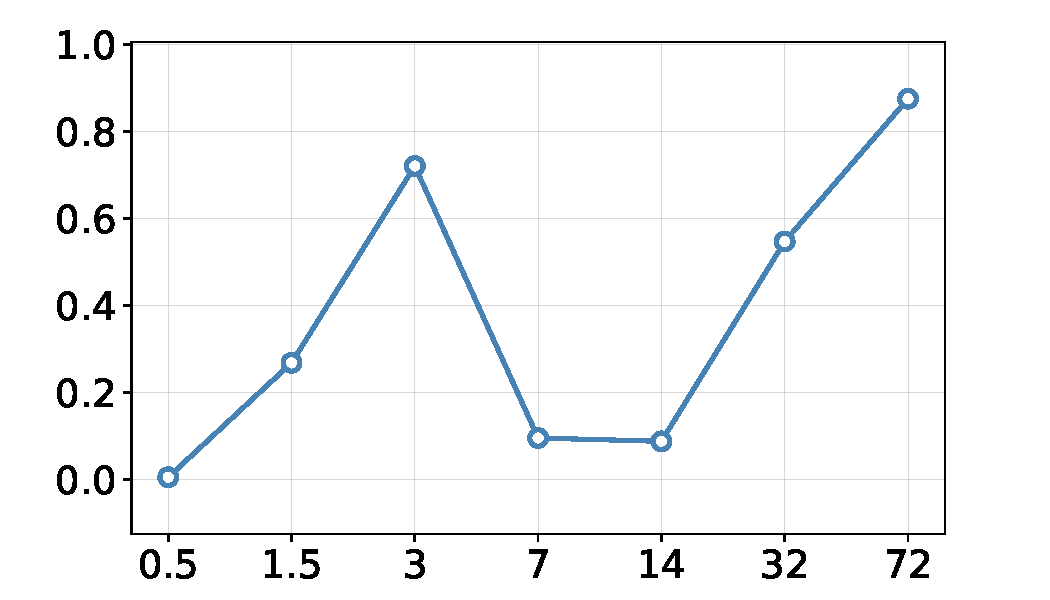
\includegraphics[width=\linewidth]{Figures_Qwen_scaling/GSM8k__..pdf}
        \caption{Resp. = "."}
    \end{subfigure}
    \hfill
    \begin{subfigure}{0.3\textwidth}
        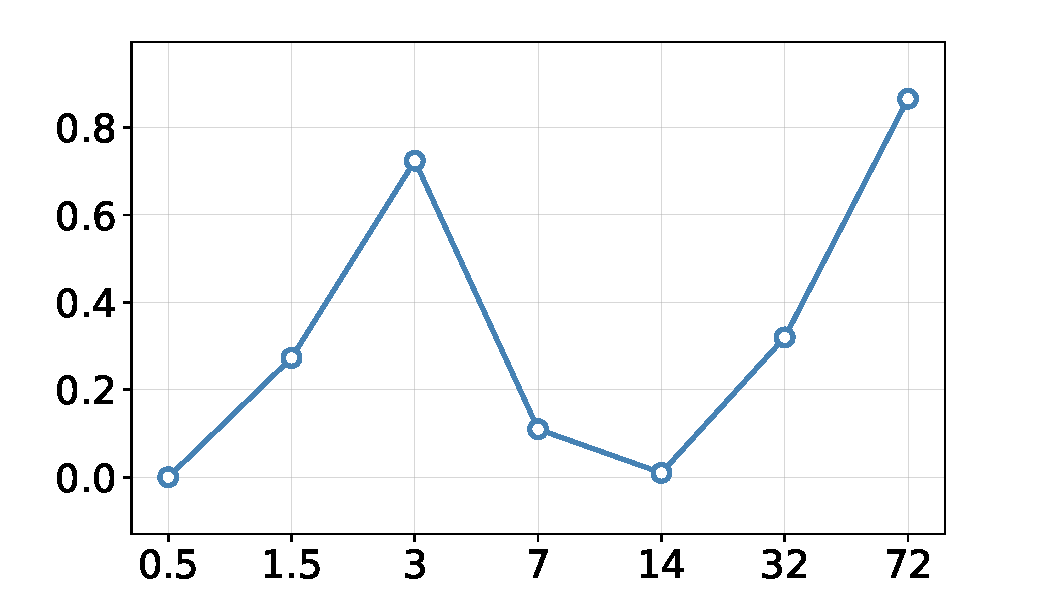
\includegraphics[width=\linewidth]{Figures_Qwen_scaling/GSM8k__,.pdf}
        \caption{Resp. = ","}
    \end{subfigure}
    
    \vspace{0.5em}
    % second row
    \begin{subfigure}{0.3\textwidth}
        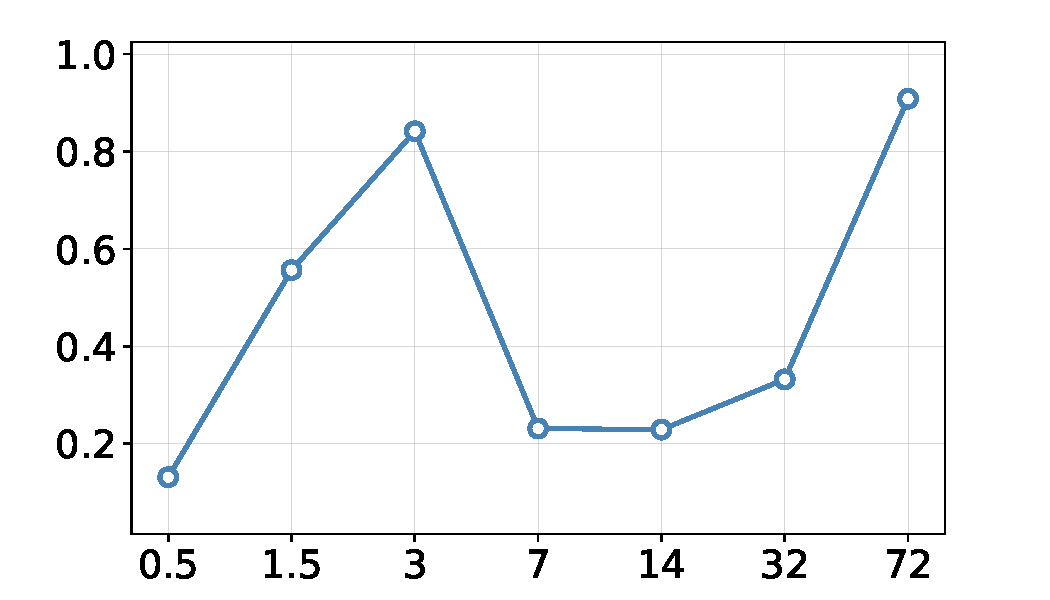
\includegraphics[width=\linewidth]{Figures_Qwen_scaling/GSM8k__colon.pdf}
        \caption{Resp. = ":"}
    \end{subfigure}
    \hfill
    \begin{subfigure}{0.3\textwidth}
        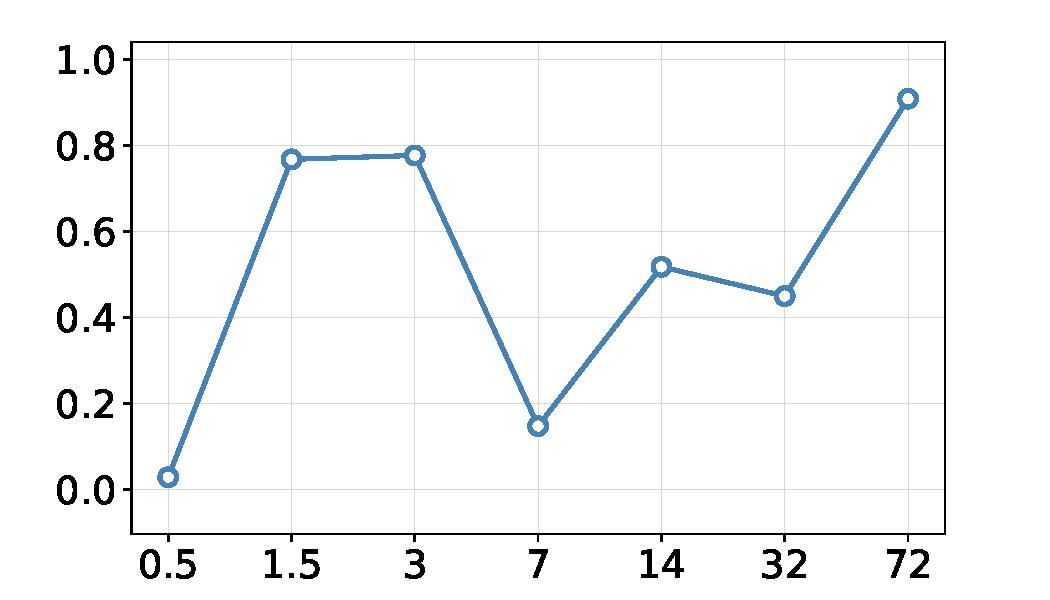
\includegraphics[width=\linewidth]{Figures_Qwen_scaling/GSM8k__Thought_processcolon.pdf}
        \caption{Resp. = "Thought process:"}
    \end{subfigure}
    \hfill
    \begin{subfigure}{0.3\textwidth}
        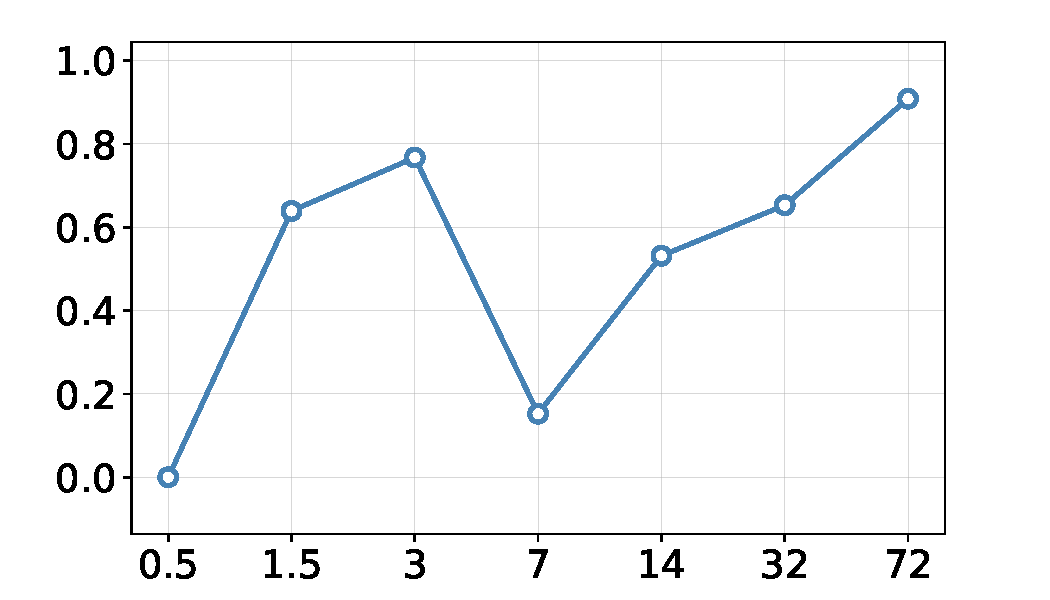
\includegraphics[width=\linewidth]{Figures_Qwen_scaling/GSM8k__Let_solve_this_problem_step_by_step..pdf}
        \caption{Resp. = "Let's solve this problem step by step"}
    \end{subfigure}
    
    \vspace{0.5em}
    % third row
    \begin{subfigure}{0.22\textwidth}
        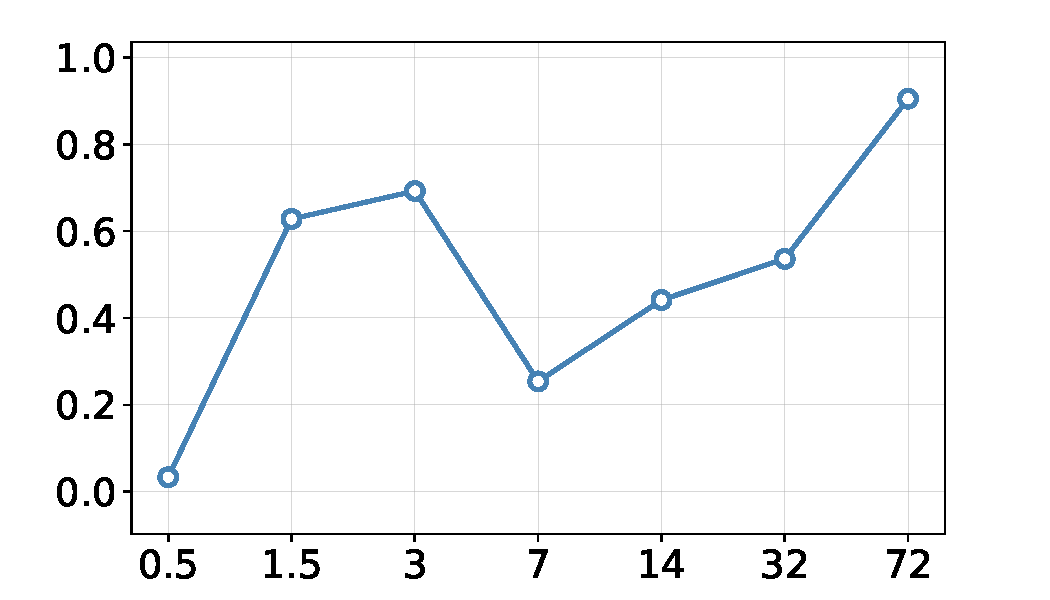
\includegraphics[width=\linewidth]{Figures_Qwen_scaling/GSM8k__Solution.pdf}
        \caption{Resp. = "Solution"}
    \end{subfigure}
    \hfill
    \begin{subfigure}{0.22\textwidth}
        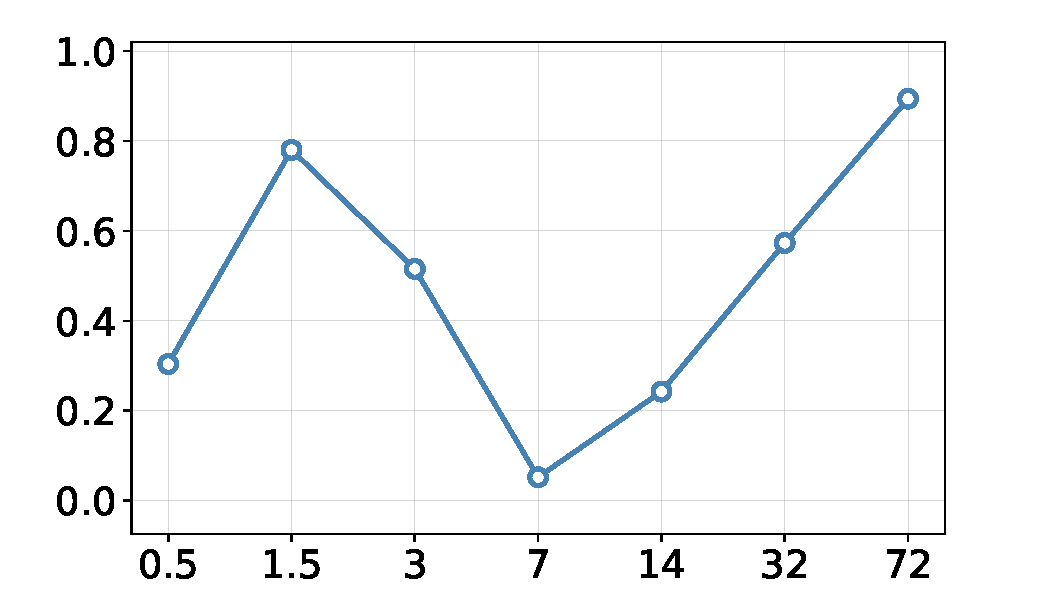
\includegraphics[width=\linewidth]{Figures_Qwen_scaling/GSM8k__china.pdf}
        \caption{Resp. = "\begin{CJK}{UTF8}{gbsn}解\end{CJK}"}
    \end{subfigure}
    \hfill
    \begin{subfigure}{0.22\textwidth}
        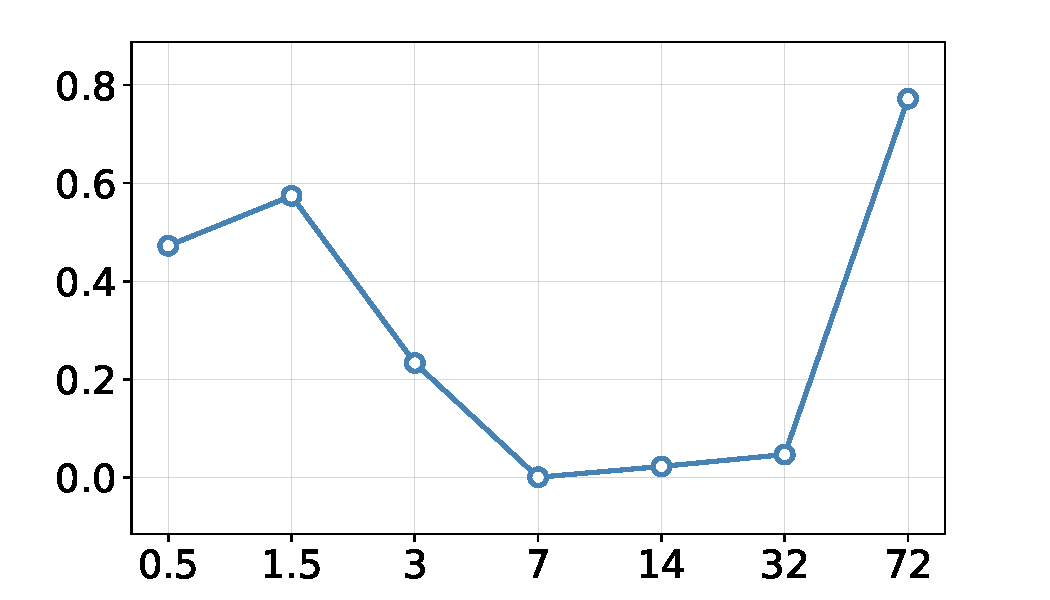
\includegraphics[width=\linewidth]{Figures_Qwen_scaling/GSM8k__jap.pdf}
        \caption{Resp. = \begin{CJK}{UTF8}{min}かいせつ\end{CJK}}
    \end{subfigure}
    \hfill
    \begin{subfigure}{0.22\textwidth}
        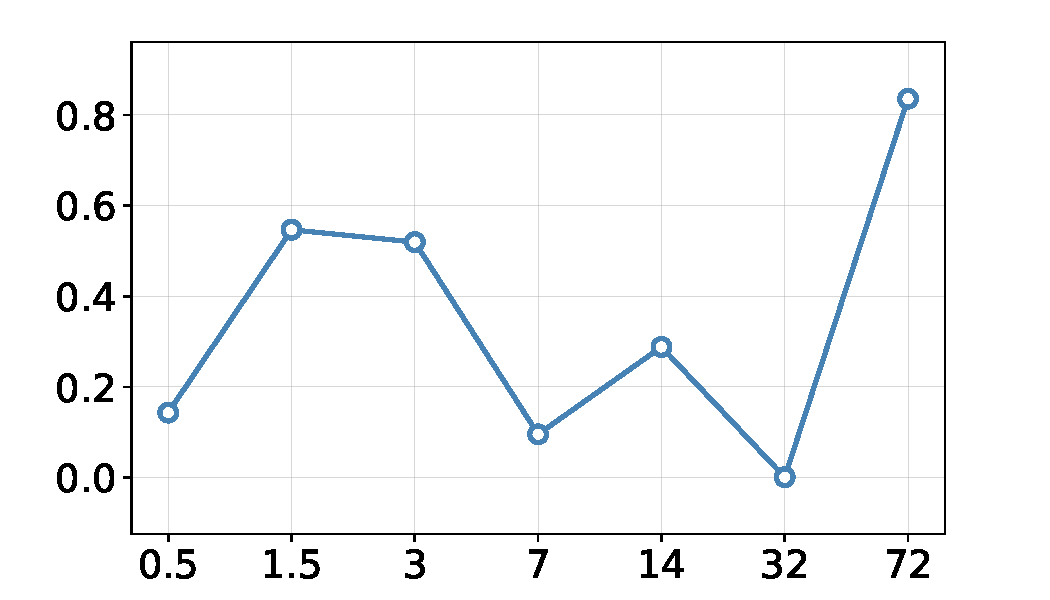
\includegraphics[width=\linewidth]{Figures_Qwen_scaling/GSM8k__Respuesta.pdf}
        \caption{Resp. = \foreignlanguage{spanish}{Respuesta}}
    \end{subfigure}
    
    \caption{GSM8K Benchmark}
    \label{fig:ten_gsm8k}
\end{figure*}



\begin{figure*}[htbp]
    \centering
    % first row
    \begin{subfigure}{0.3\textwidth}
        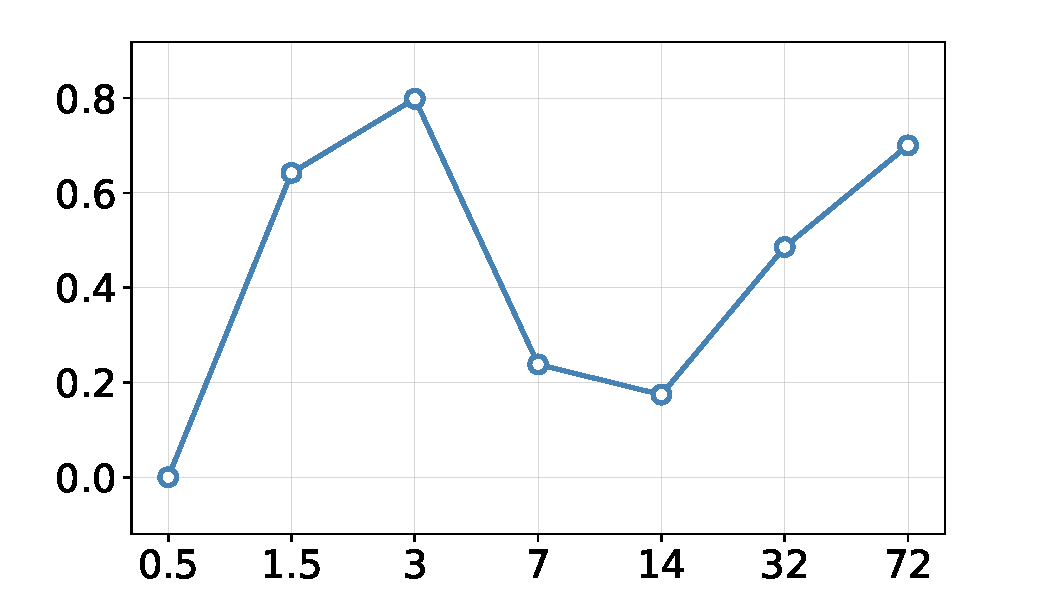
\includegraphics[width=\linewidth]{Figures_Qwen_scaling/MATH___.pdf}
        \caption{Resp. = " "}
    \end{subfigure}
    \hfill
    \begin{subfigure}{0.3\textwidth}
        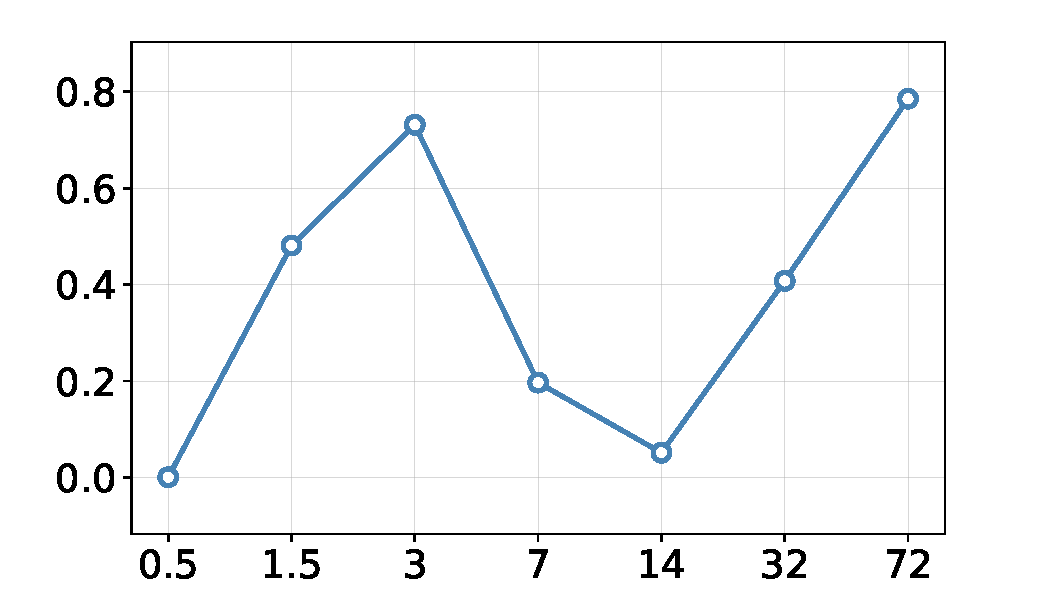
\includegraphics[width=\linewidth]{Figures_Qwen_scaling/MATH__..pdf}
        \caption{Resp. = "."}
    \end{subfigure}
    \hfill
    \begin{subfigure}{0.3\textwidth}
        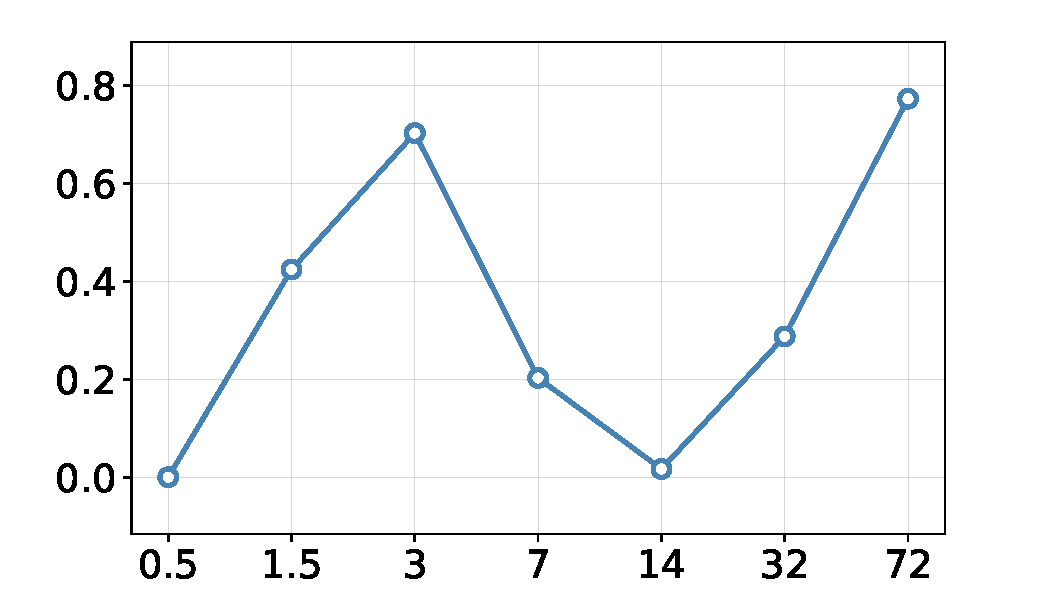
\includegraphics[width=\linewidth]{Figures_Qwen_scaling/MATH__,.pdf}
        \caption{Resp. = ","}
    \end{subfigure}
    
    \vspace{0.5em}
    % second row
    \begin{subfigure}{0.3\textwidth}
        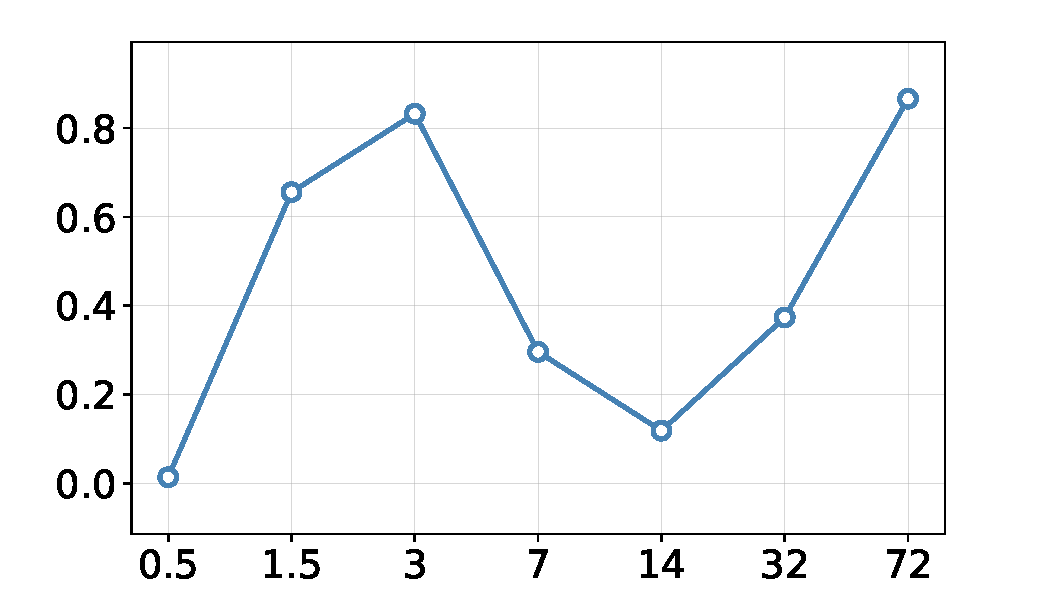
\includegraphics[width=\linewidth]{Figures_Qwen_scaling/MATH__colon.pdf}
        \caption{Resp. = ":"}
    \end{subfigure}
    \hfill
    \begin{subfigure}{0.3\textwidth}
        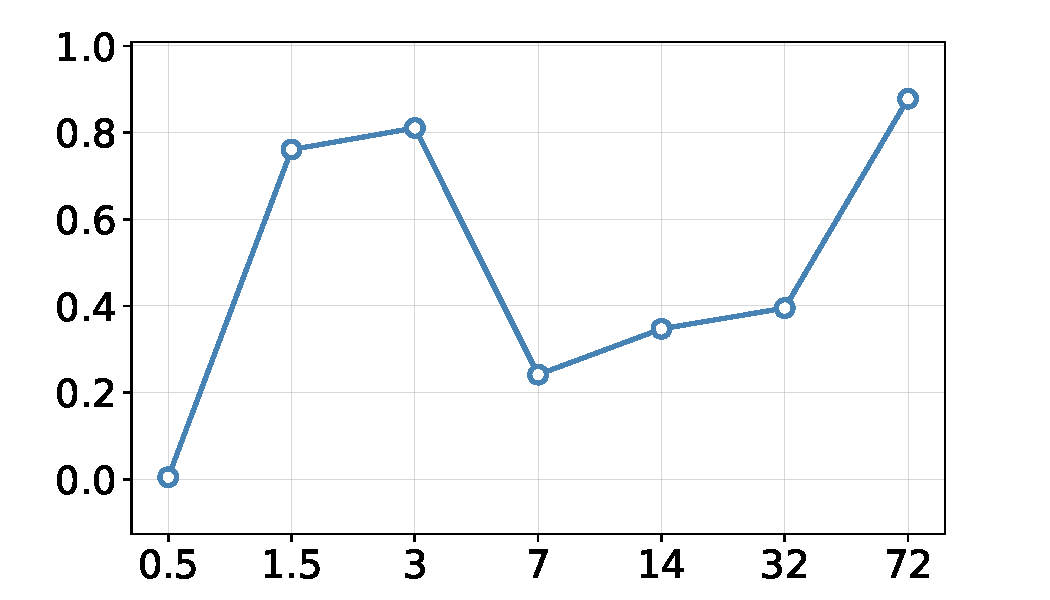
\includegraphics[width=\linewidth]{Figures_Qwen_scaling/MATH__Thought_processcolon.pdf}
        \caption{Resp. = "Thought process:"}
    \end{subfigure}
    \hfill
    \begin{subfigure}{0.3\textwidth}
        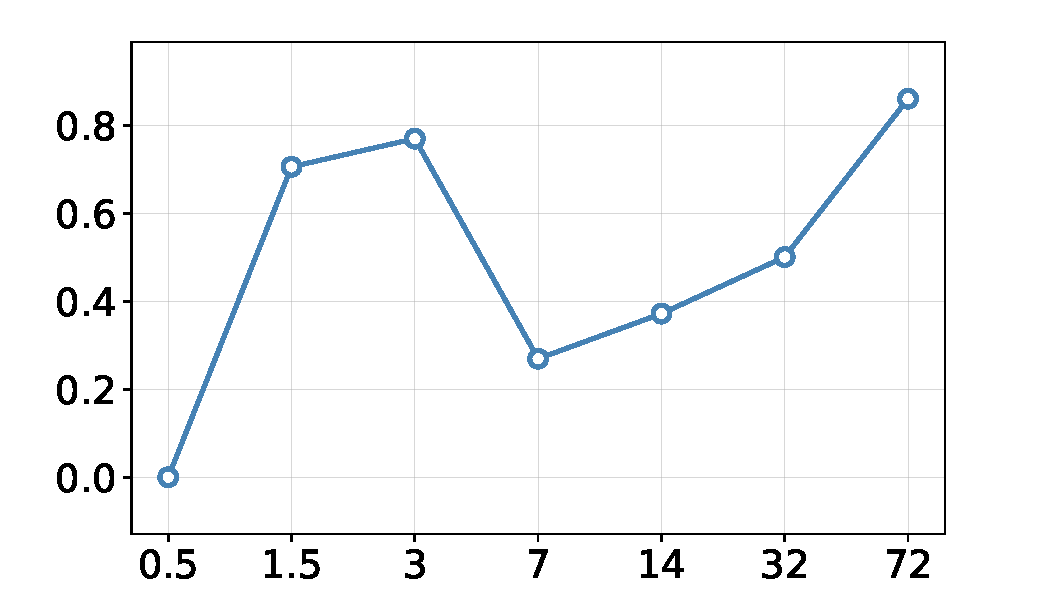
\includegraphics[width=\linewidth]{Figures_Qwen_scaling/MATH__Let_solve_this_problem_step_by_step..pdf}
        \caption{Resp. = "Let's solve this problem step by step"}
    \end{subfigure}
    
    \vspace{0.5em}
    % third row
    \begin{subfigure}{0.22\textwidth}
        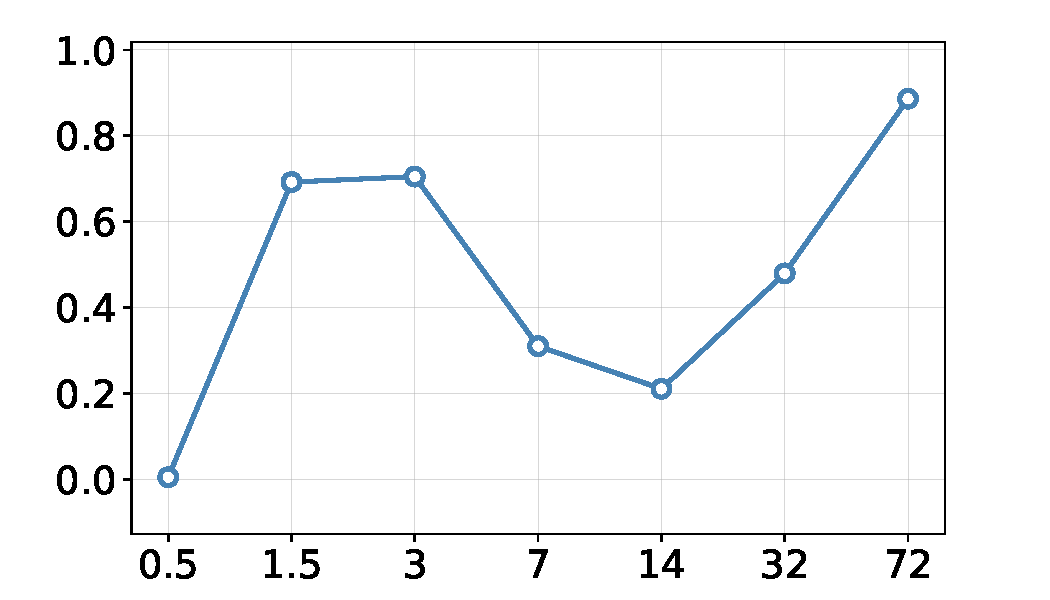
\includegraphics[width=\linewidth]{Figures_Qwen_scaling/MATH__Solution.pdf}
        \caption{Resp. = "Solution"}
    \end{subfigure}
    \hfill
    \begin{subfigure}{0.22\textwidth}
        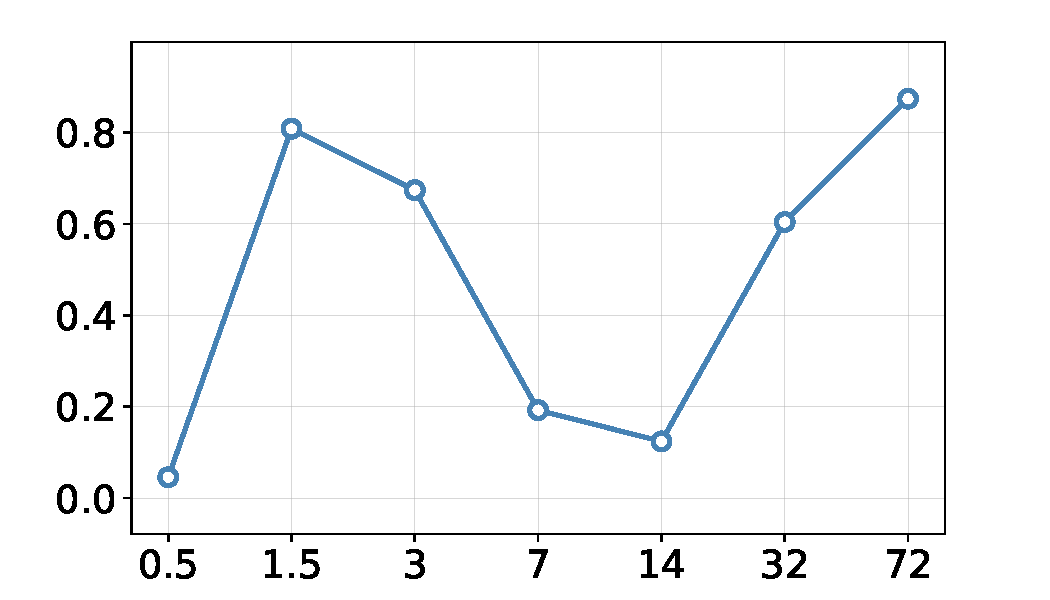
\includegraphics[width=\linewidth]{Figures_Qwen_scaling/MATH__china.pdf}
        \caption{Resp. = "\begin{CJK}{UTF8}{gbsn}解\end{CJK}"}
    \end{subfigure}
    \hfill
    \begin{subfigure}{0.22\textwidth}
        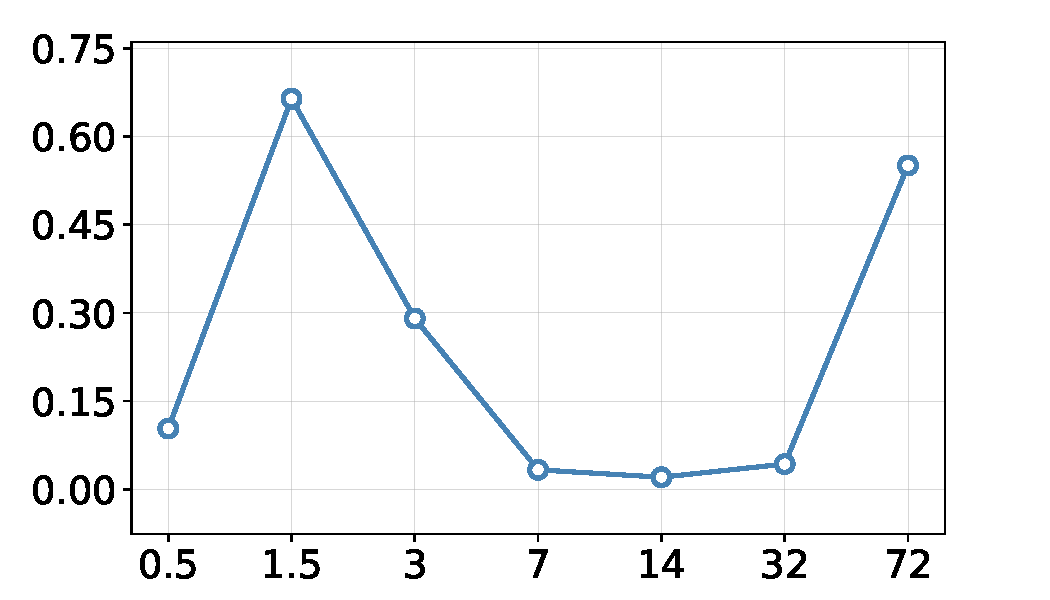
\includegraphics[width=\linewidth]{Figures_Qwen_scaling/MATH__jap.pdf}
        \caption{Resp. = \begin{CJK}{UTF8}{min}かいせつ\end{CJK}}
    \end{subfigure}
    \hfill
    \begin{subfigure}{0.22\textwidth}
        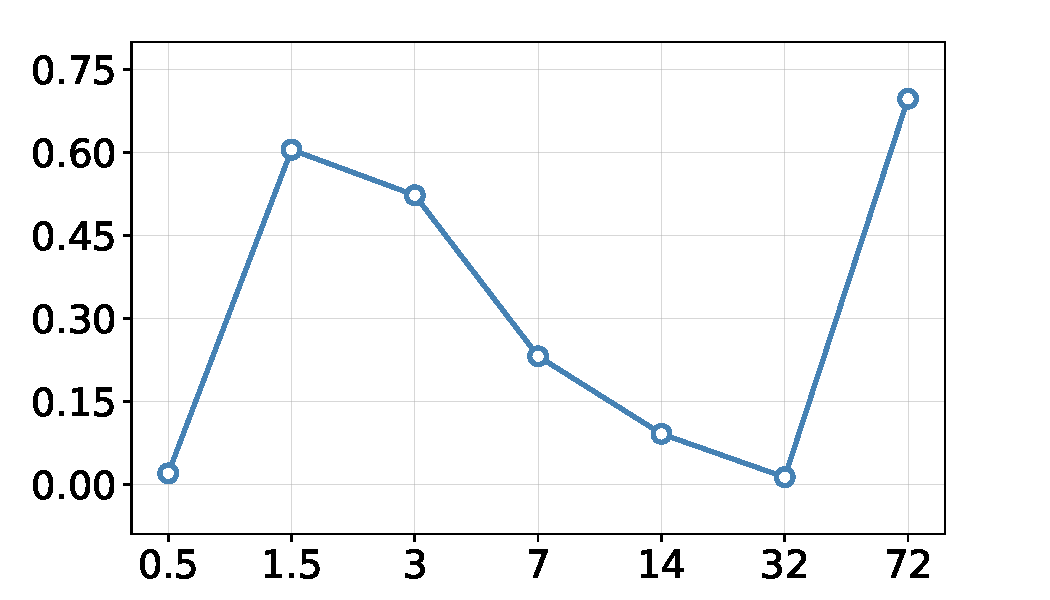
\includegraphics[width=\linewidth]{Figures_Qwen_scaling/MATH__Respuesta.pdf}
        \caption{Resp. = \foreignlanguage{spanish}{Respuesta}}
    \end{subfigure}
    
    \caption{MATH Benchmark}
    \label{fig:ten_math}
\end{figure*}




\begin{figure*}[htbp]
    \centering
    % first row
    \begin{subfigure}{0.3\textwidth}
        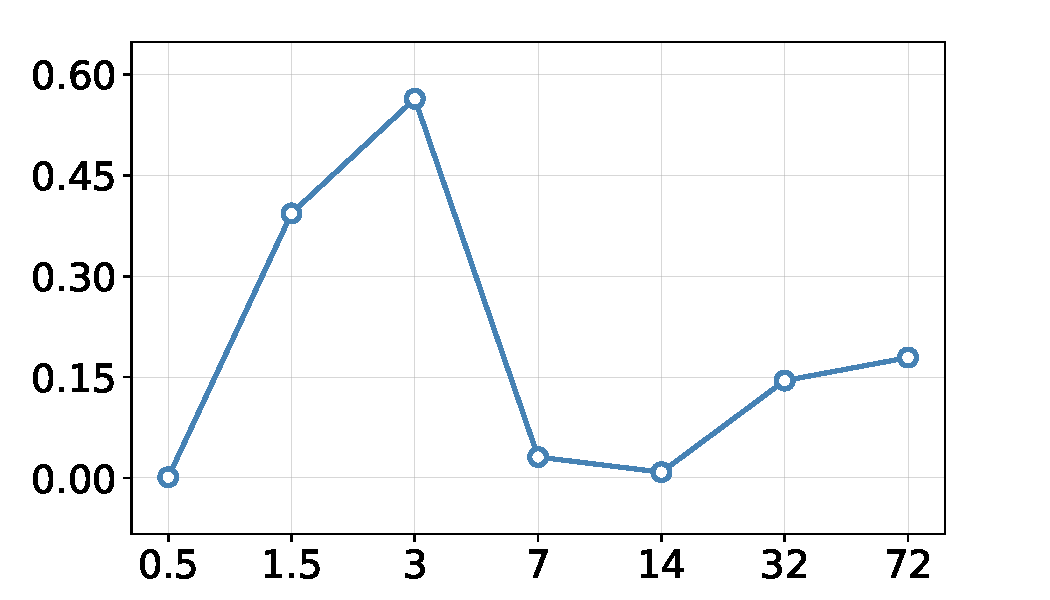
\includegraphics[width=\linewidth]{Figures_Qwen_scaling/AIME1983-2024___.pdf}
        \caption{Resp. = " "}
    \end{subfigure}
    \hfill
    \begin{subfigure}{0.3\textwidth}
        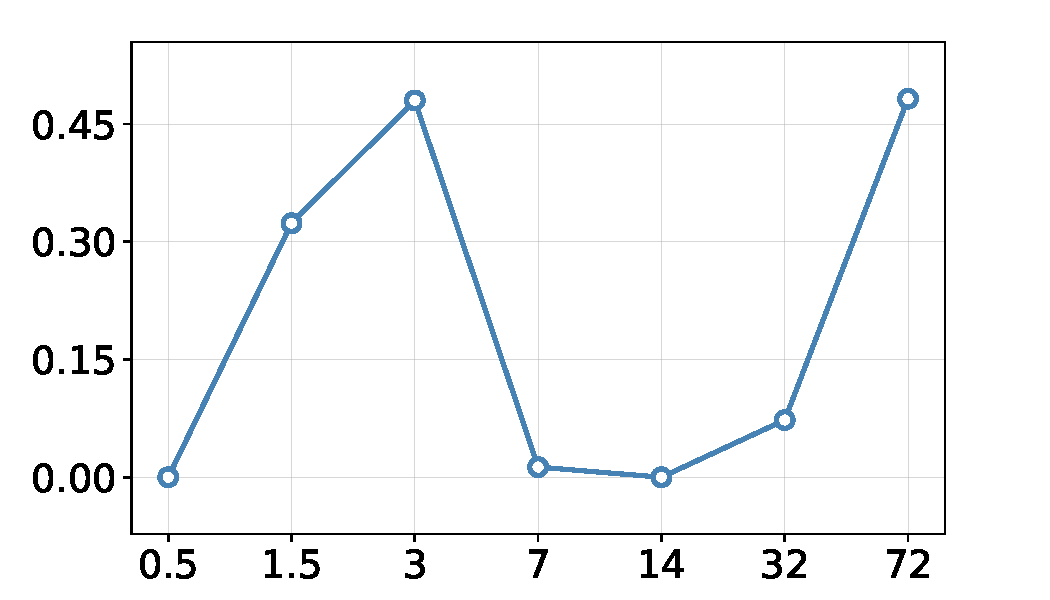
\includegraphics[width=\linewidth]{Figures_Qwen_scaling/AIME1983-2024__..pdf}
        \caption{Resp. = "."}
    \end{subfigure}
    \hfill
    \begin{subfigure}{0.3\textwidth}
        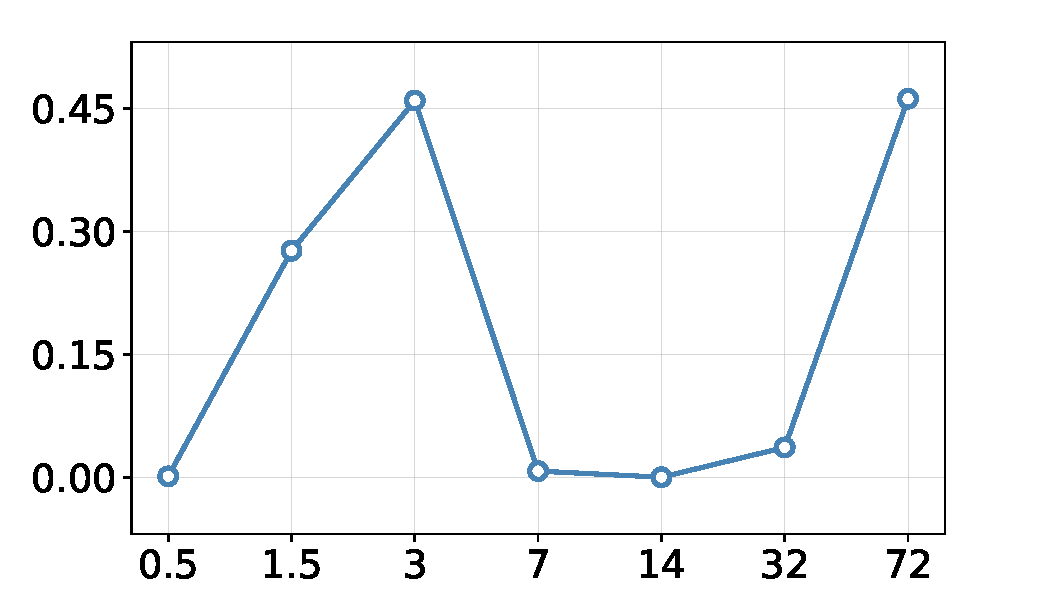
\includegraphics[width=\linewidth]{Figures_Qwen_scaling/AIME1983-2024__,.pdf}
        \caption{Resp. = ","}
    \end{subfigure}
    
    \vspace{0.5em}
    % second row
    \begin{subfigure}{0.3\textwidth}
        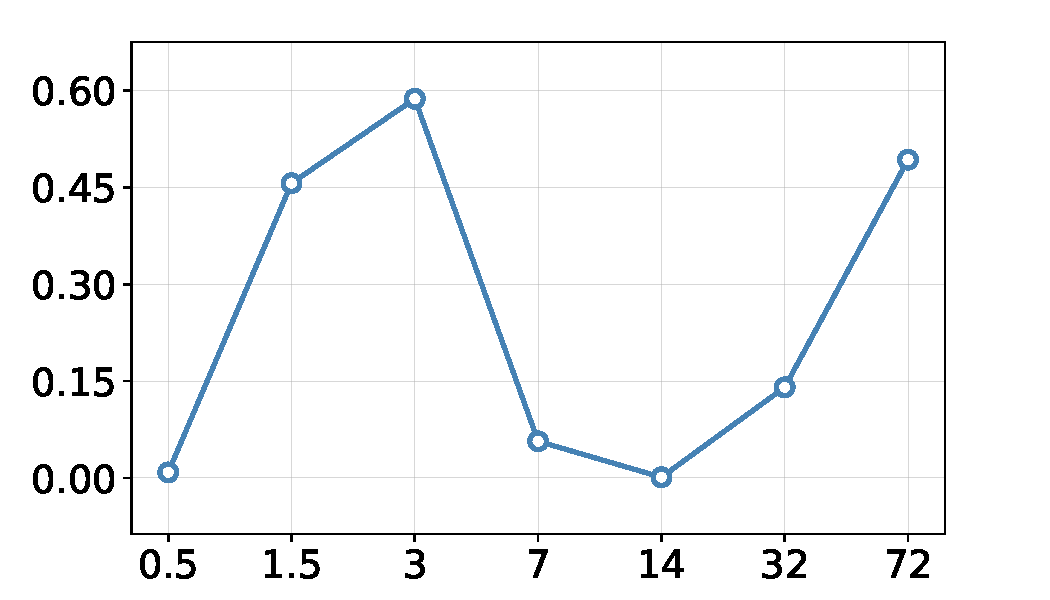
\includegraphics[width=\linewidth]{Figures_Qwen_scaling/AIME1983-2024__colon.pdf}
        \caption{Resp. = ":"}
    \end{subfigure}
    \hfill
    \begin{subfigure}{0.3\textwidth}
        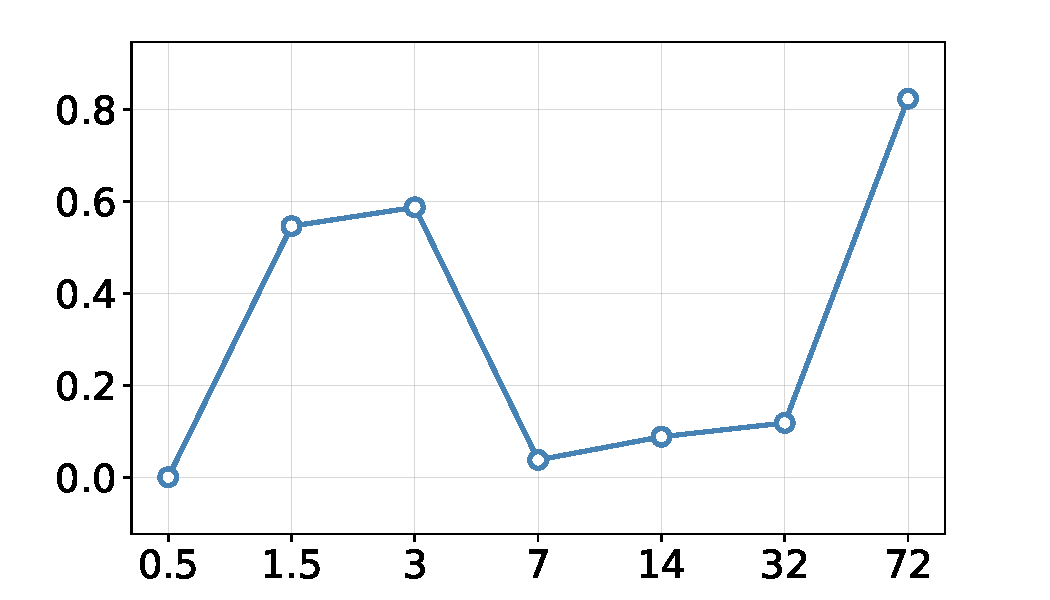
\includegraphics[width=\linewidth]{Figures_Qwen_scaling/AIME1983-2024__Thought_processcolon.pdf}
        \caption{Resp. = "Thought process:"}
    \end{subfigure}
    \hfill
    \begin{subfigure}{0.3\textwidth}
        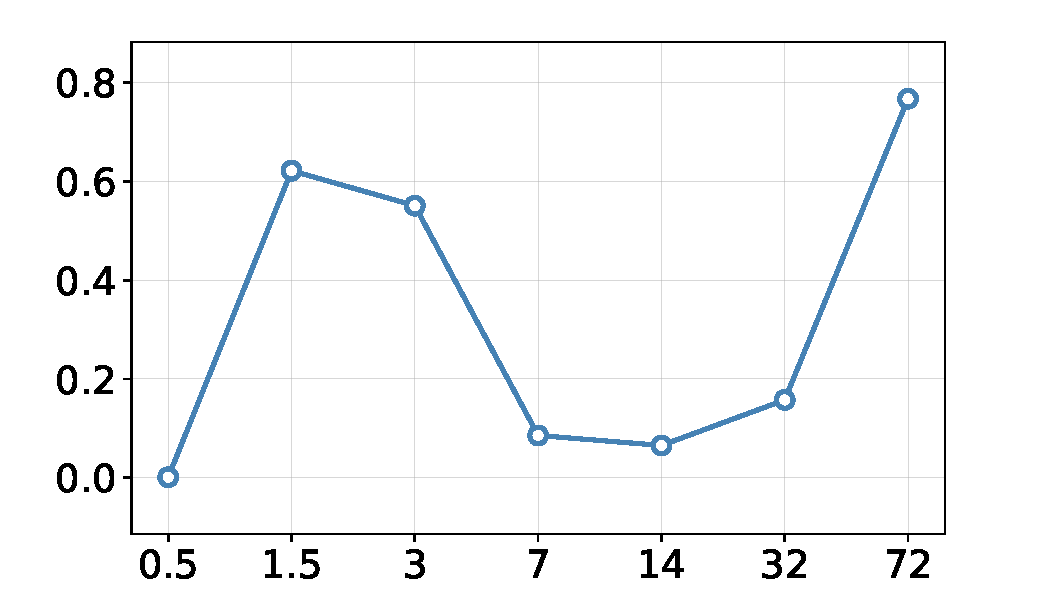
\includegraphics[width=\linewidth]{Figures_Qwen_scaling/AIME1983-2024__Let_solve_this_problem_step_by_step..pdf}
        \caption{Resp. = "Let's solve this problem step by step"}
    \end{subfigure}
    
    \vspace{0.5em}
    % third row
    \begin{subfigure}{0.22\textwidth}
        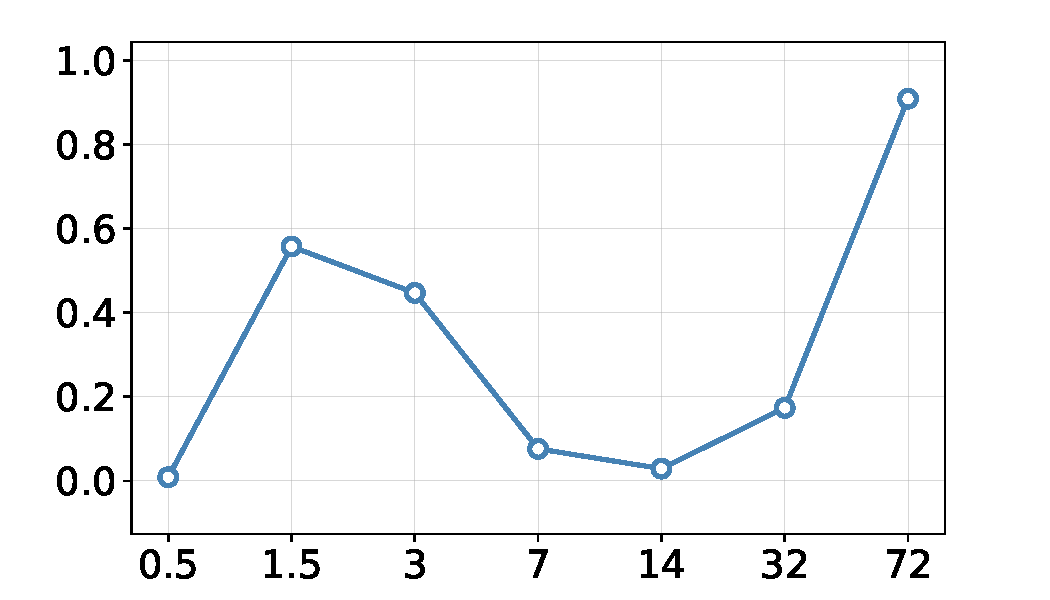
\includegraphics[width=\linewidth]{Figures_Qwen_scaling/AIME1983-2024__Solution.pdf}
        \caption{Resp. = "Solution"}
    \end{subfigure}
    \hfill
    \begin{subfigure}{0.22\textwidth}
        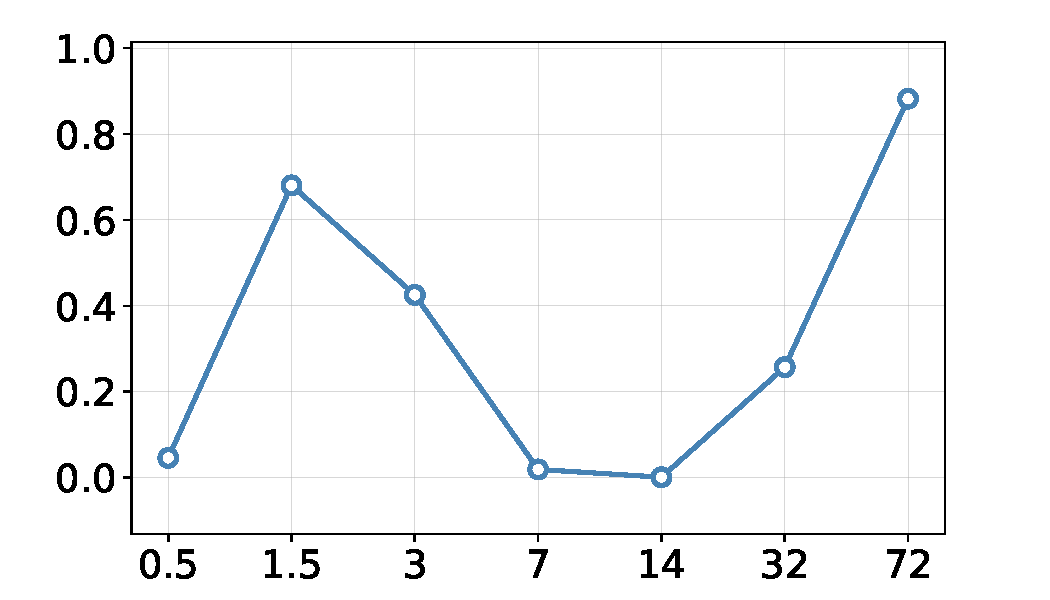
\includegraphics[width=\linewidth]{Figures_Qwen_scaling/AIME1983-2024__china.pdf}
        \caption{Resp. = "\begin{CJK}{UTF8}{gbsn}解\end{CJK}"}
    \end{subfigure}
    \hfill
    \begin{subfigure}{0.22\textwidth}
        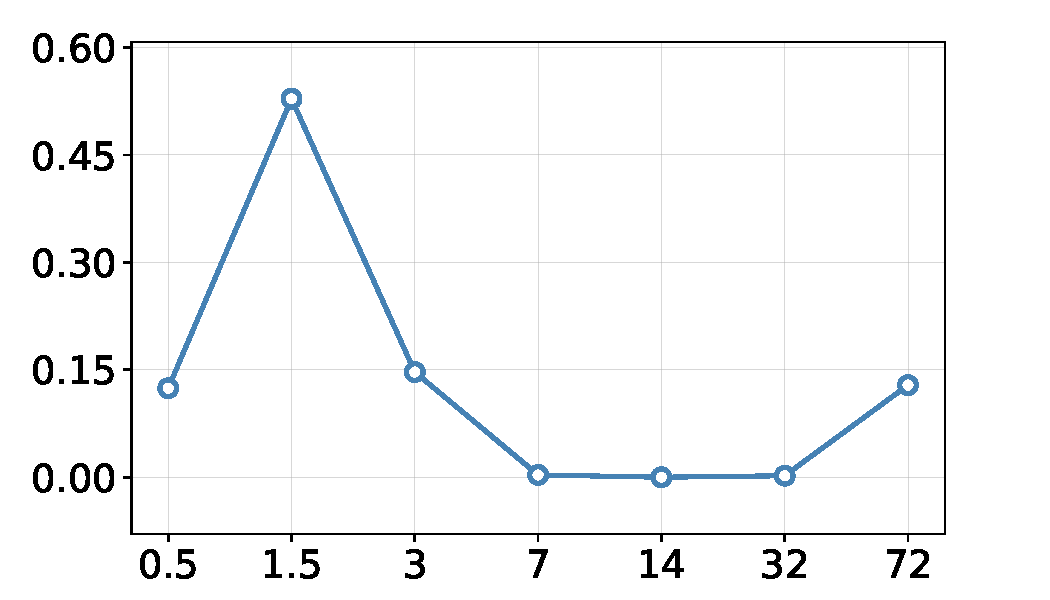
\includegraphics[width=\linewidth]{Figures_Qwen_scaling/AIME1983-2024__jap.pdf}
        \caption{Resp. = \begin{CJK}{UTF8}{min}かいせつ\end{CJK}}
    \end{subfigure}
    \hfill
    \begin{subfigure}{0.22\textwidth}
        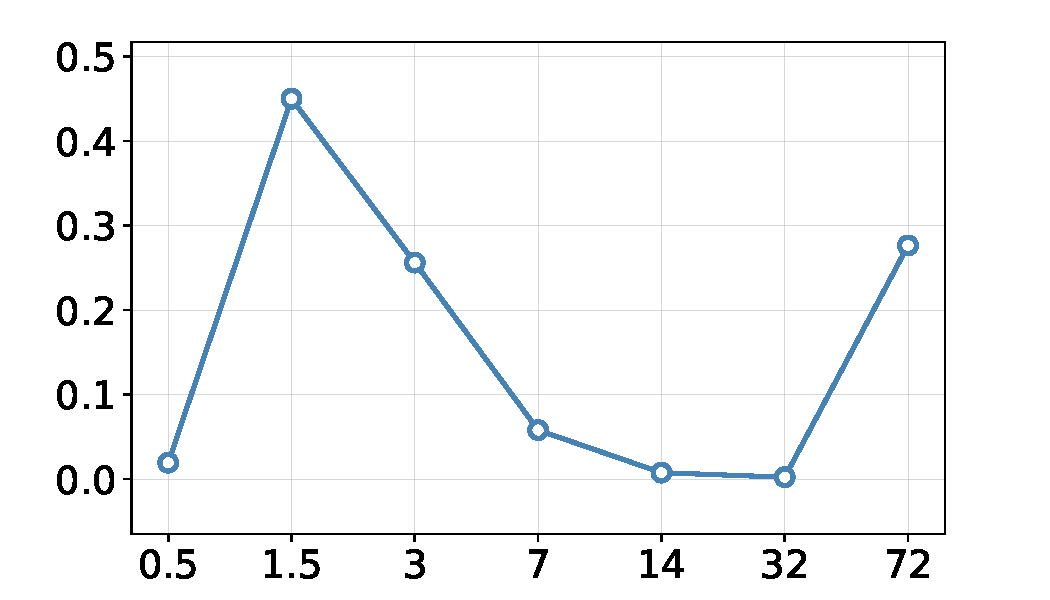
\includegraphics[width=\linewidth]{Figures_Qwen_scaling/AIME1983-2024__Respuesta.pdf}
        \caption{Resp. = \foreignlanguage{spanish}{Respuesta}}
    \end{subfigure}
    
    \caption{AIME1983-2024 Benchmark}
    \label{fig:ten_aime}
\end{figure*}


